\documentclass[12pt,]{article}
\usepackage[left=1in,top=1in,right=1in,bottom=1in]{geometry}
\newcommand*{\authorfont}{\fontfamily{phv}\selectfont}
\usepackage[]{mathpazo}


  \usepackage[T1]{fontenc}
  \usepackage[utf8]{inputenc}



\usepackage{abstract}
\renewcommand{\abstractname}{}    % clear the title
\renewcommand{\absnamepos}{empty} % originally center

\renewenvironment{abstract}
 {{%
    \setlength{\leftmargin}{0mm}
    \setlength{\rightmargin}{\leftmargin}%
  }%
  \relax}
 {\endlist}

\makeatletter
\def\@maketitle{%
  \newpage
%  \null
%  \vskip 2em%
%  \begin{center}%
  \let \footnote \thanks
    {\fontsize{18}{20}\selectfont\raggedright  \setlength{\parindent}{0pt} \@title \par}%
}
%\fi
\makeatother




\setcounter{secnumdepth}{0}


\usepackage{graphicx,grffile}
\makeatletter
\def\maxwidth{\ifdim\Gin@nat@width>\linewidth\linewidth\else\Gin@nat@width\fi}
\def\maxheight{\ifdim\Gin@nat@height>\textheight\textheight\else\Gin@nat@height\fi}
\makeatother
% Scale images if necessary, so that they will not overflow the page
% margins by default, and it is still possible to overwrite the defaults
% using explicit options in \includegraphics[width, height, ...]{}
\setkeys{Gin}{width=\maxwidth,height=\maxheight,keepaspectratio}

\title{Social Closeness and Dishonesty \thanks{Replication files are available on the author's Github account
\url{https://github.com/saidejp/social_closeness}}  }



\author{\Large Said E. Jiménez\vspace{0.05in} \newline\normalsize\emph{Universidad Nacional Autónoma de México}   \and \Large Roberto Mercadillo\vspace{0.05in} \newline\normalsize\emph{Universidad Autónoma Metropolitana}   \and \Large Eduardo Garza-Villarreal\vspace{0.05in} \newline\normalsize\emph{Instituto Nacional de Psiquiatría Ramón de la Fuente Muñiz}  }


\date{}

\usepackage{titlesec}

\titleformat*{\section}{\normalsize\bfseries}
\titleformat*{\subsection}{\normalsize\itshape}
\titleformat*{\subsubsection}{\normalsize\itshape}
\titleformat*{\paragraph}{\normalsize\itshape}
\titleformat*{\subparagraph}{\normalsize\itshape}


\usepackage{natbib}
\bibliographystyle{apsr}
\usepackage[strings]{underscore} % protect underscores in most circumstances



\newtheorem{hypothesis}{Hypothesis}
\usepackage{setspace}

\makeatletter
\@ifpackageloaded{hyperref}{}{%
\ifxetex
  \PassOptionsToPackage{hyphens}{url}\usepackage[setpagesize=false, % page size defined by xetex
              unicode=false, % unicode breaks when used with xetex
              xetex]{hyperref}
\else
  \PassOptionsToPackage{hyphens}{url}\usepackage[unicode=true]{hyperref}
\fi
}

\@ifpackageloaded{color}{
    \PassOptionsToPackage{usenames,dvipsnames}{color}
}{%
    \usepackage[usenames,dvipsnames]{color}
}
\makeatother
\hypersetup{breaklinks=true,
            bookmarks=true,
            pdfauthor={Said E. Jiménez (Universidad Nacional Autónoma de México) and Roberto Mercadillo (Universidad Autónoma Metropolitana) and Eduardo Garza-Villarreal (Instituto Nacional de Psiquiatría Ramón de la Fuente Muñiz)},
             pdfkeywords = {dishonesty, bayesian hierarchical modeling, mixture modeling},  
            pdftitle={Social Closeness and Dishonesty},
            colorlinks=true,
            citecolor=blue,
            urlcolor=blue,
            linkcolor=magenta,
            pdfborder={0 0 0}}
\urlstyle{same}  % don't use monospace font for urls

% set default figure placement to htbp
\makeatletter
\def\fps@figure{htbp}
\makeatother



% add tightlist ----------
\providecommand{\tightlist}{%
\setlength{\itemsep}{0pt}\setlength{\parskip}{0pt}}

\begin{document}
	
% \pagenumbering{arabic}% resets `page` counter to 1 
%
% \maketitle

{% \usefont{T1}{pnc}{m}{n}
\setlength{\parindent}{0pt}
\thispagestyle{plain}
{\fontsize{18}{20}\selectfont\raggedright 
\maketitle  % title \par  

}

{
   \vskip 13.5pt\relax \normalsize\fontsize{11}{12} 
\textbf{\authorfont Said E. Jiménez} \hskip 15pt \emph{\small Universidad Nacional Autónoma de México}   \par \textbf{\authorfont Roberto Mercadillo} \hskip 15pt \emph{\small Universidad Autónoma Metropolitana}   \par \textbf{\authorfont Eduardo Garza-Villarreal} \hskip 15pt \emph{\small Instituto Nacional de Psiquiatría Ramón de la Fuente Muñiz}   

}

}








\begin{abstract}

    \hbox{\vrule height .2pt width 39.14pc}

    \vskip 8.5pt % \small 

\noindent This document provides an introduction to R Markdown, argues for
its\ldots{}


\vskip 8.5pt \noindent \emph{Keywords}: dishonesty, bayesian hierarchical modeling, mixture modeling \par

    \hbox{\vrule height .2pt width 39.14pc}



\end{abstract}


\vskip 6.5pt


\noindent  \section{Introduction}\label{introduction}

bla bla\ldots{}

\section{Method}\label{method}

\begin{figure}
\centering
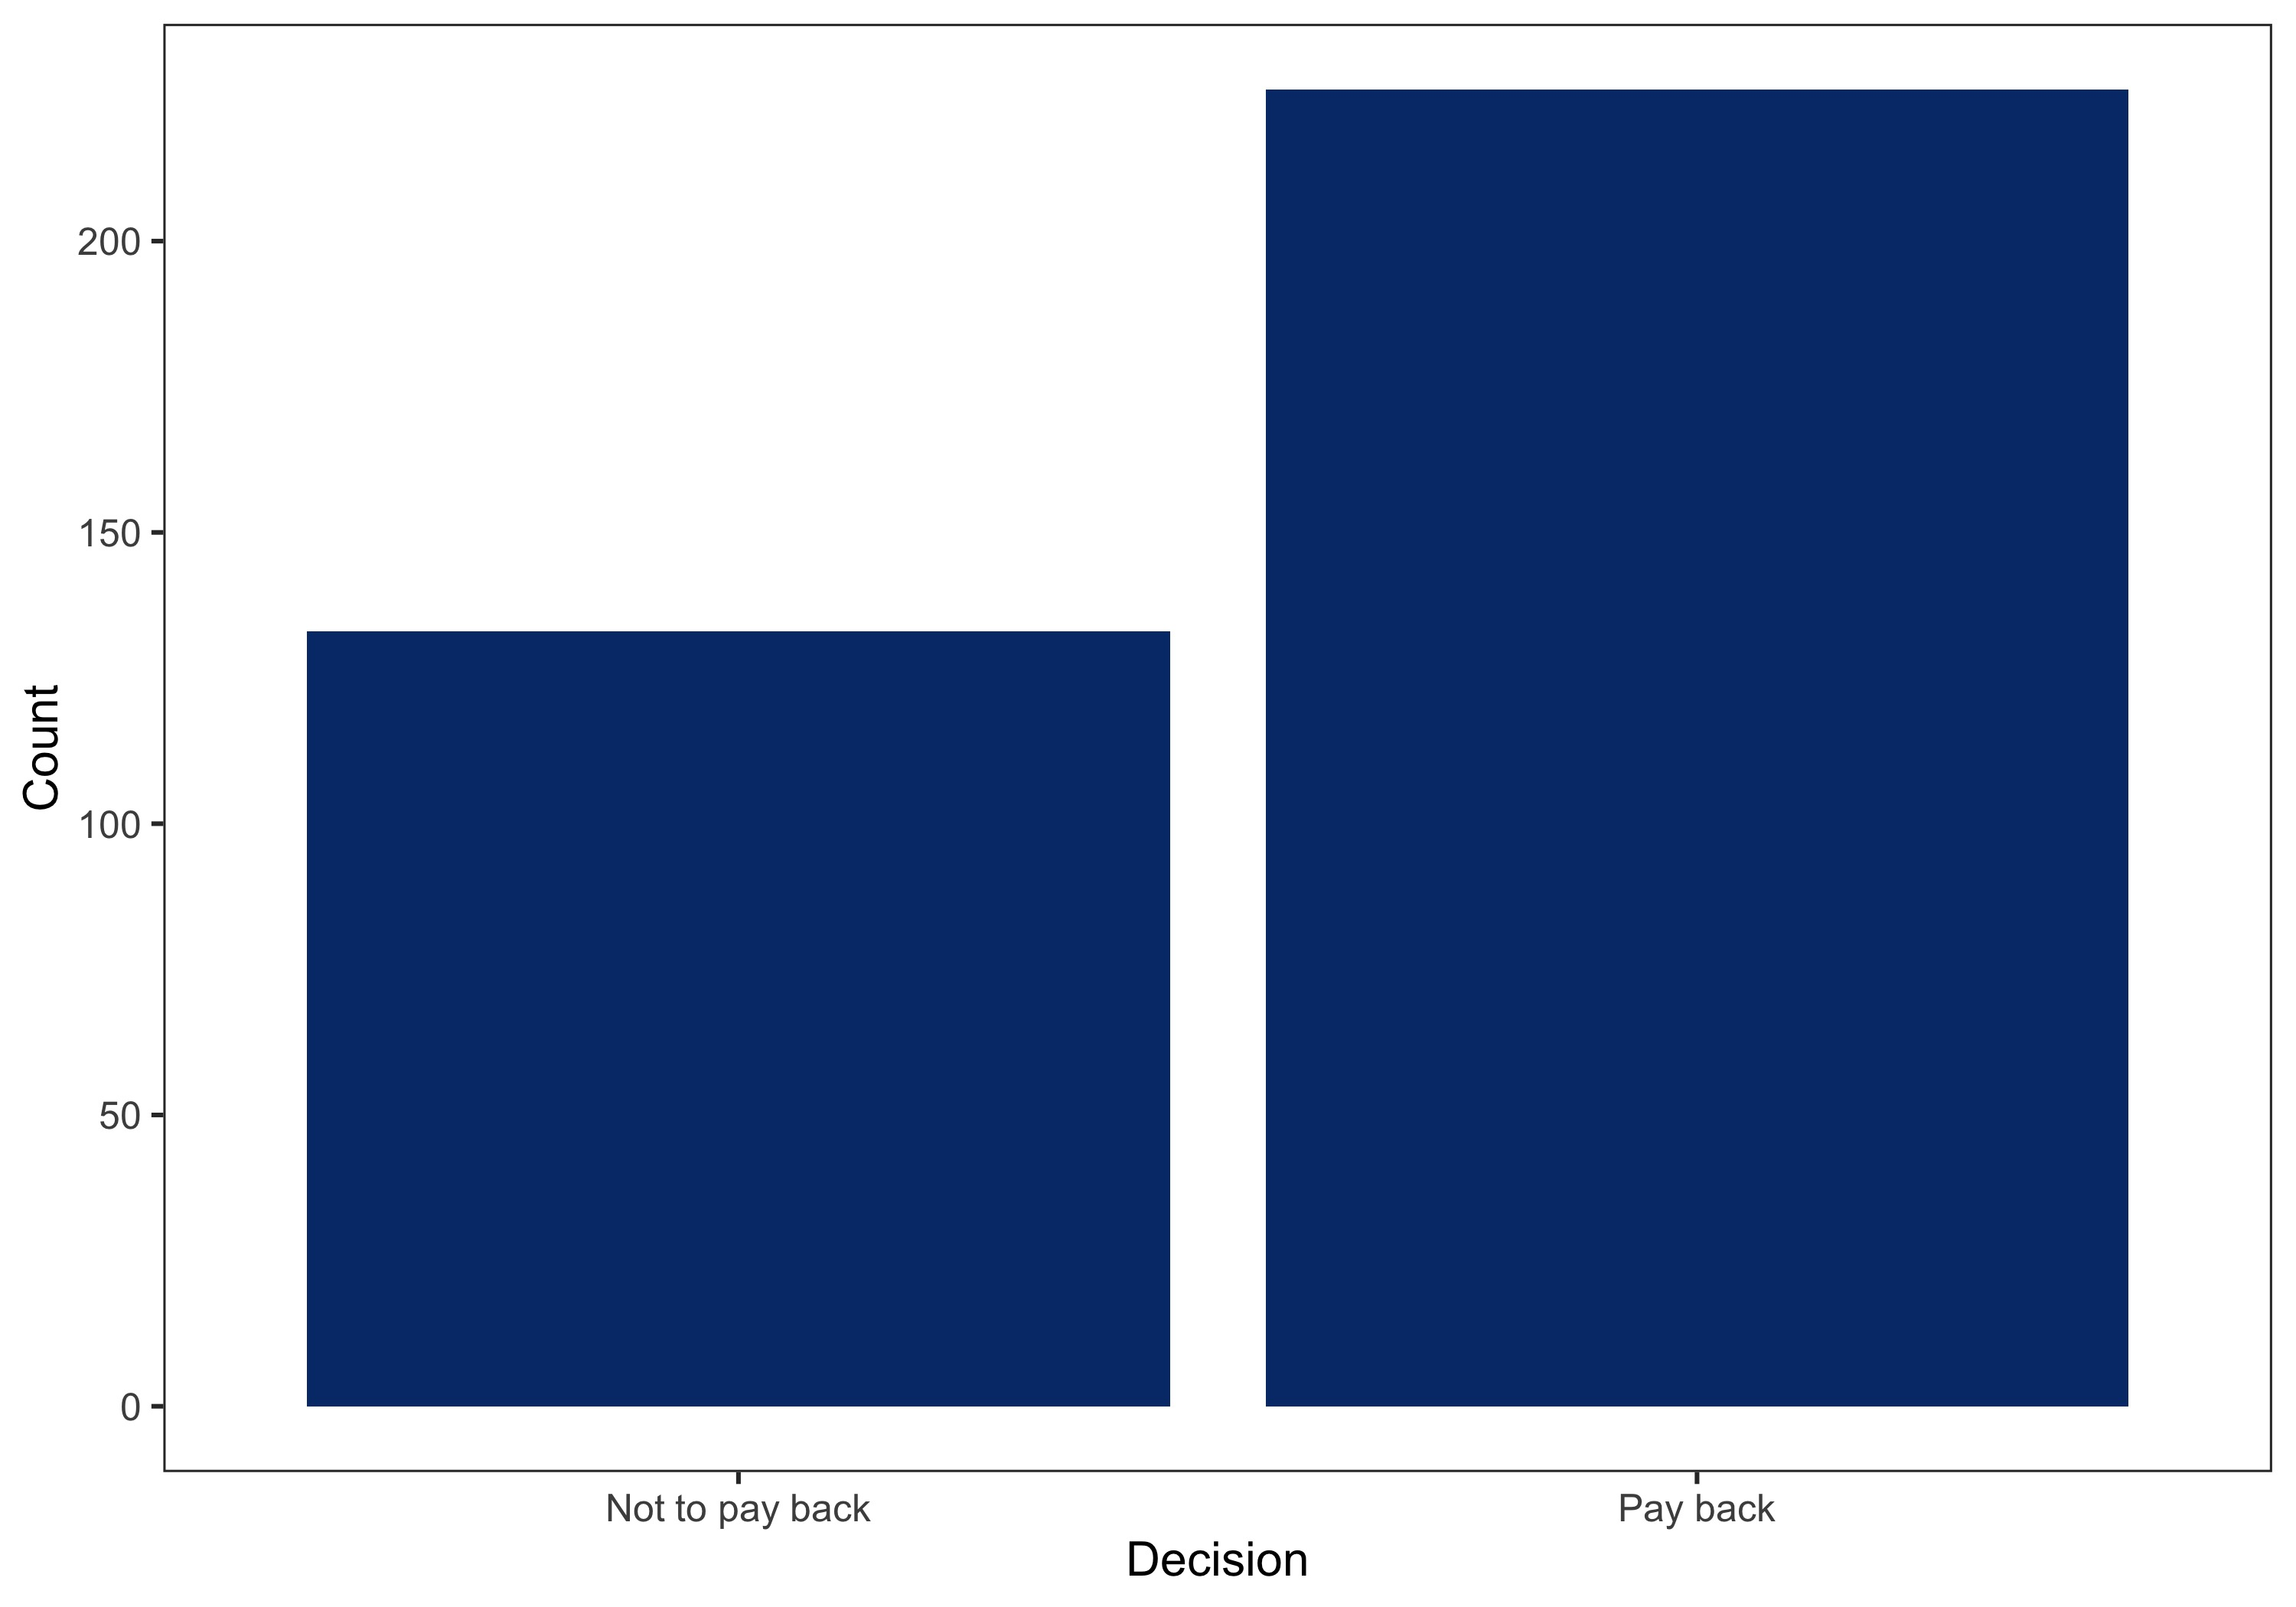
\includegraphics{/Users/saidjimenez/Documents/R/github_Said/social_closeness/Manuscript/figures/g1.jpeg}
\caption{Difference between groups in reaction time}
\end{figure}

\begin{figure}

{\centering 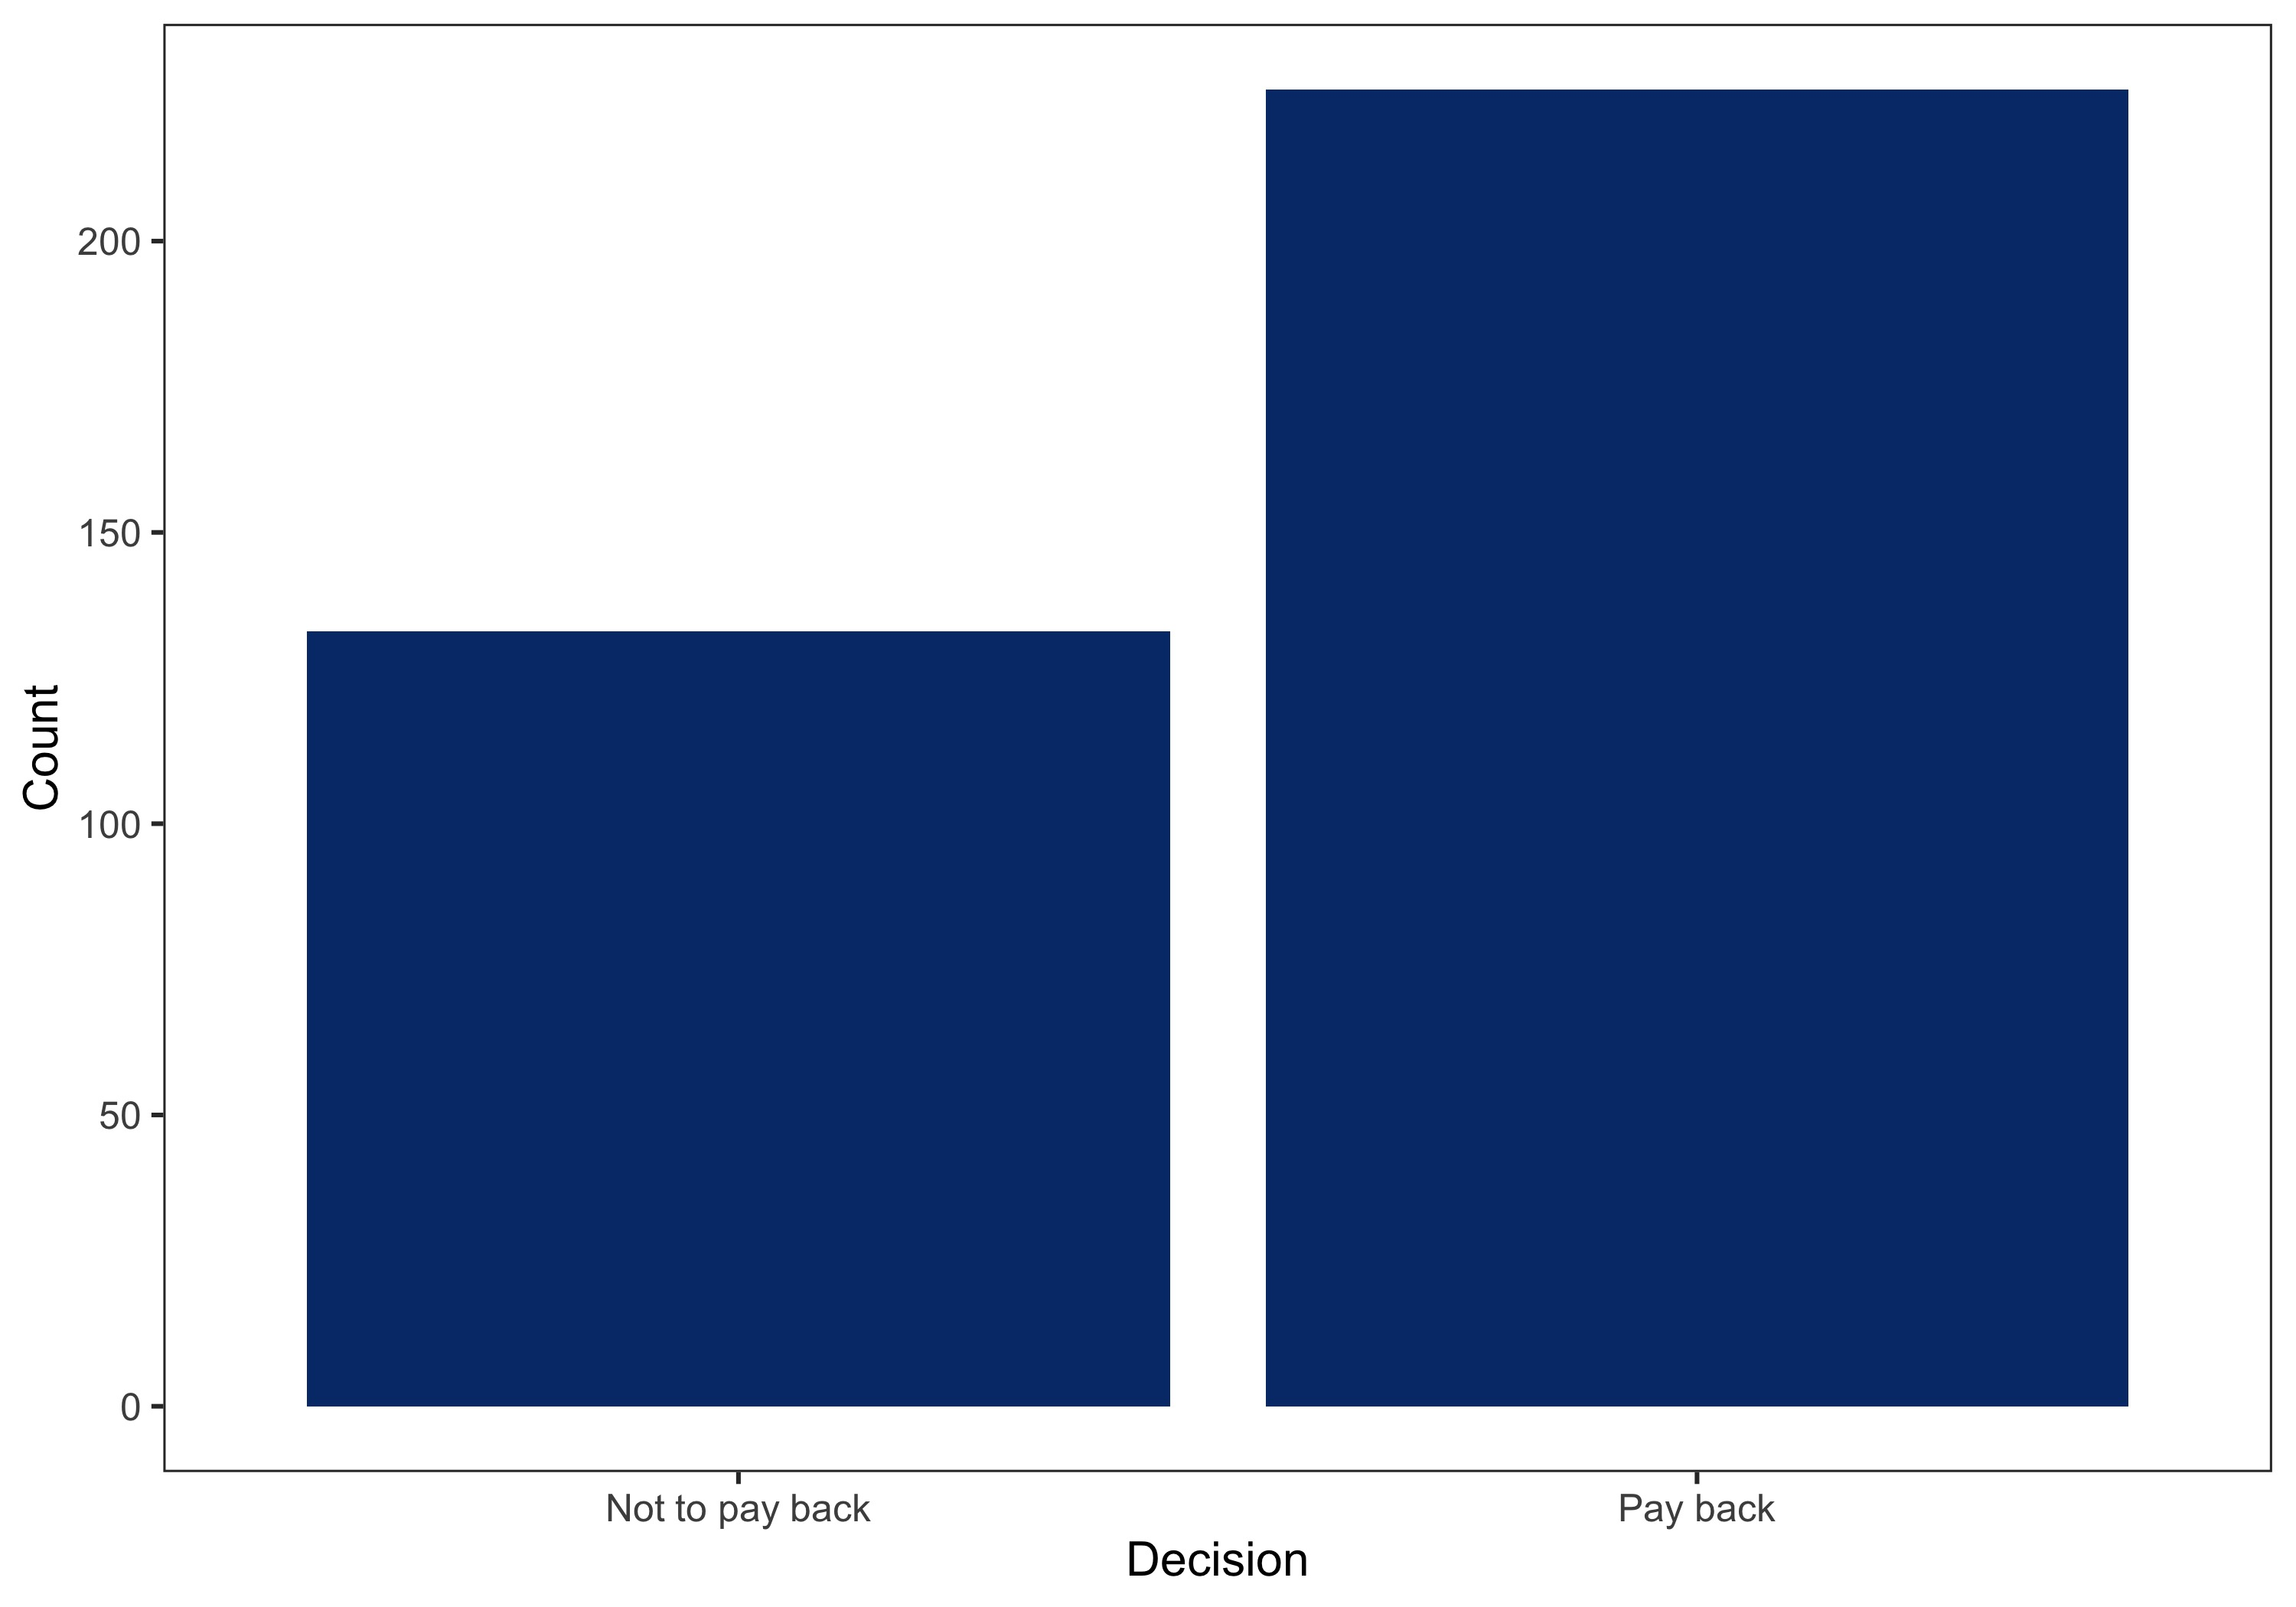
\includegraphics[width=0.8\linewidth]{/Users/saidjimenez/Documents/R/github_Said/social_closeness/Manuscript/figures/g1} 

}

\caption{Difference between groups in reaction time}\label{fig:g1}
\end{figure}

\begin{figure}

{\centering 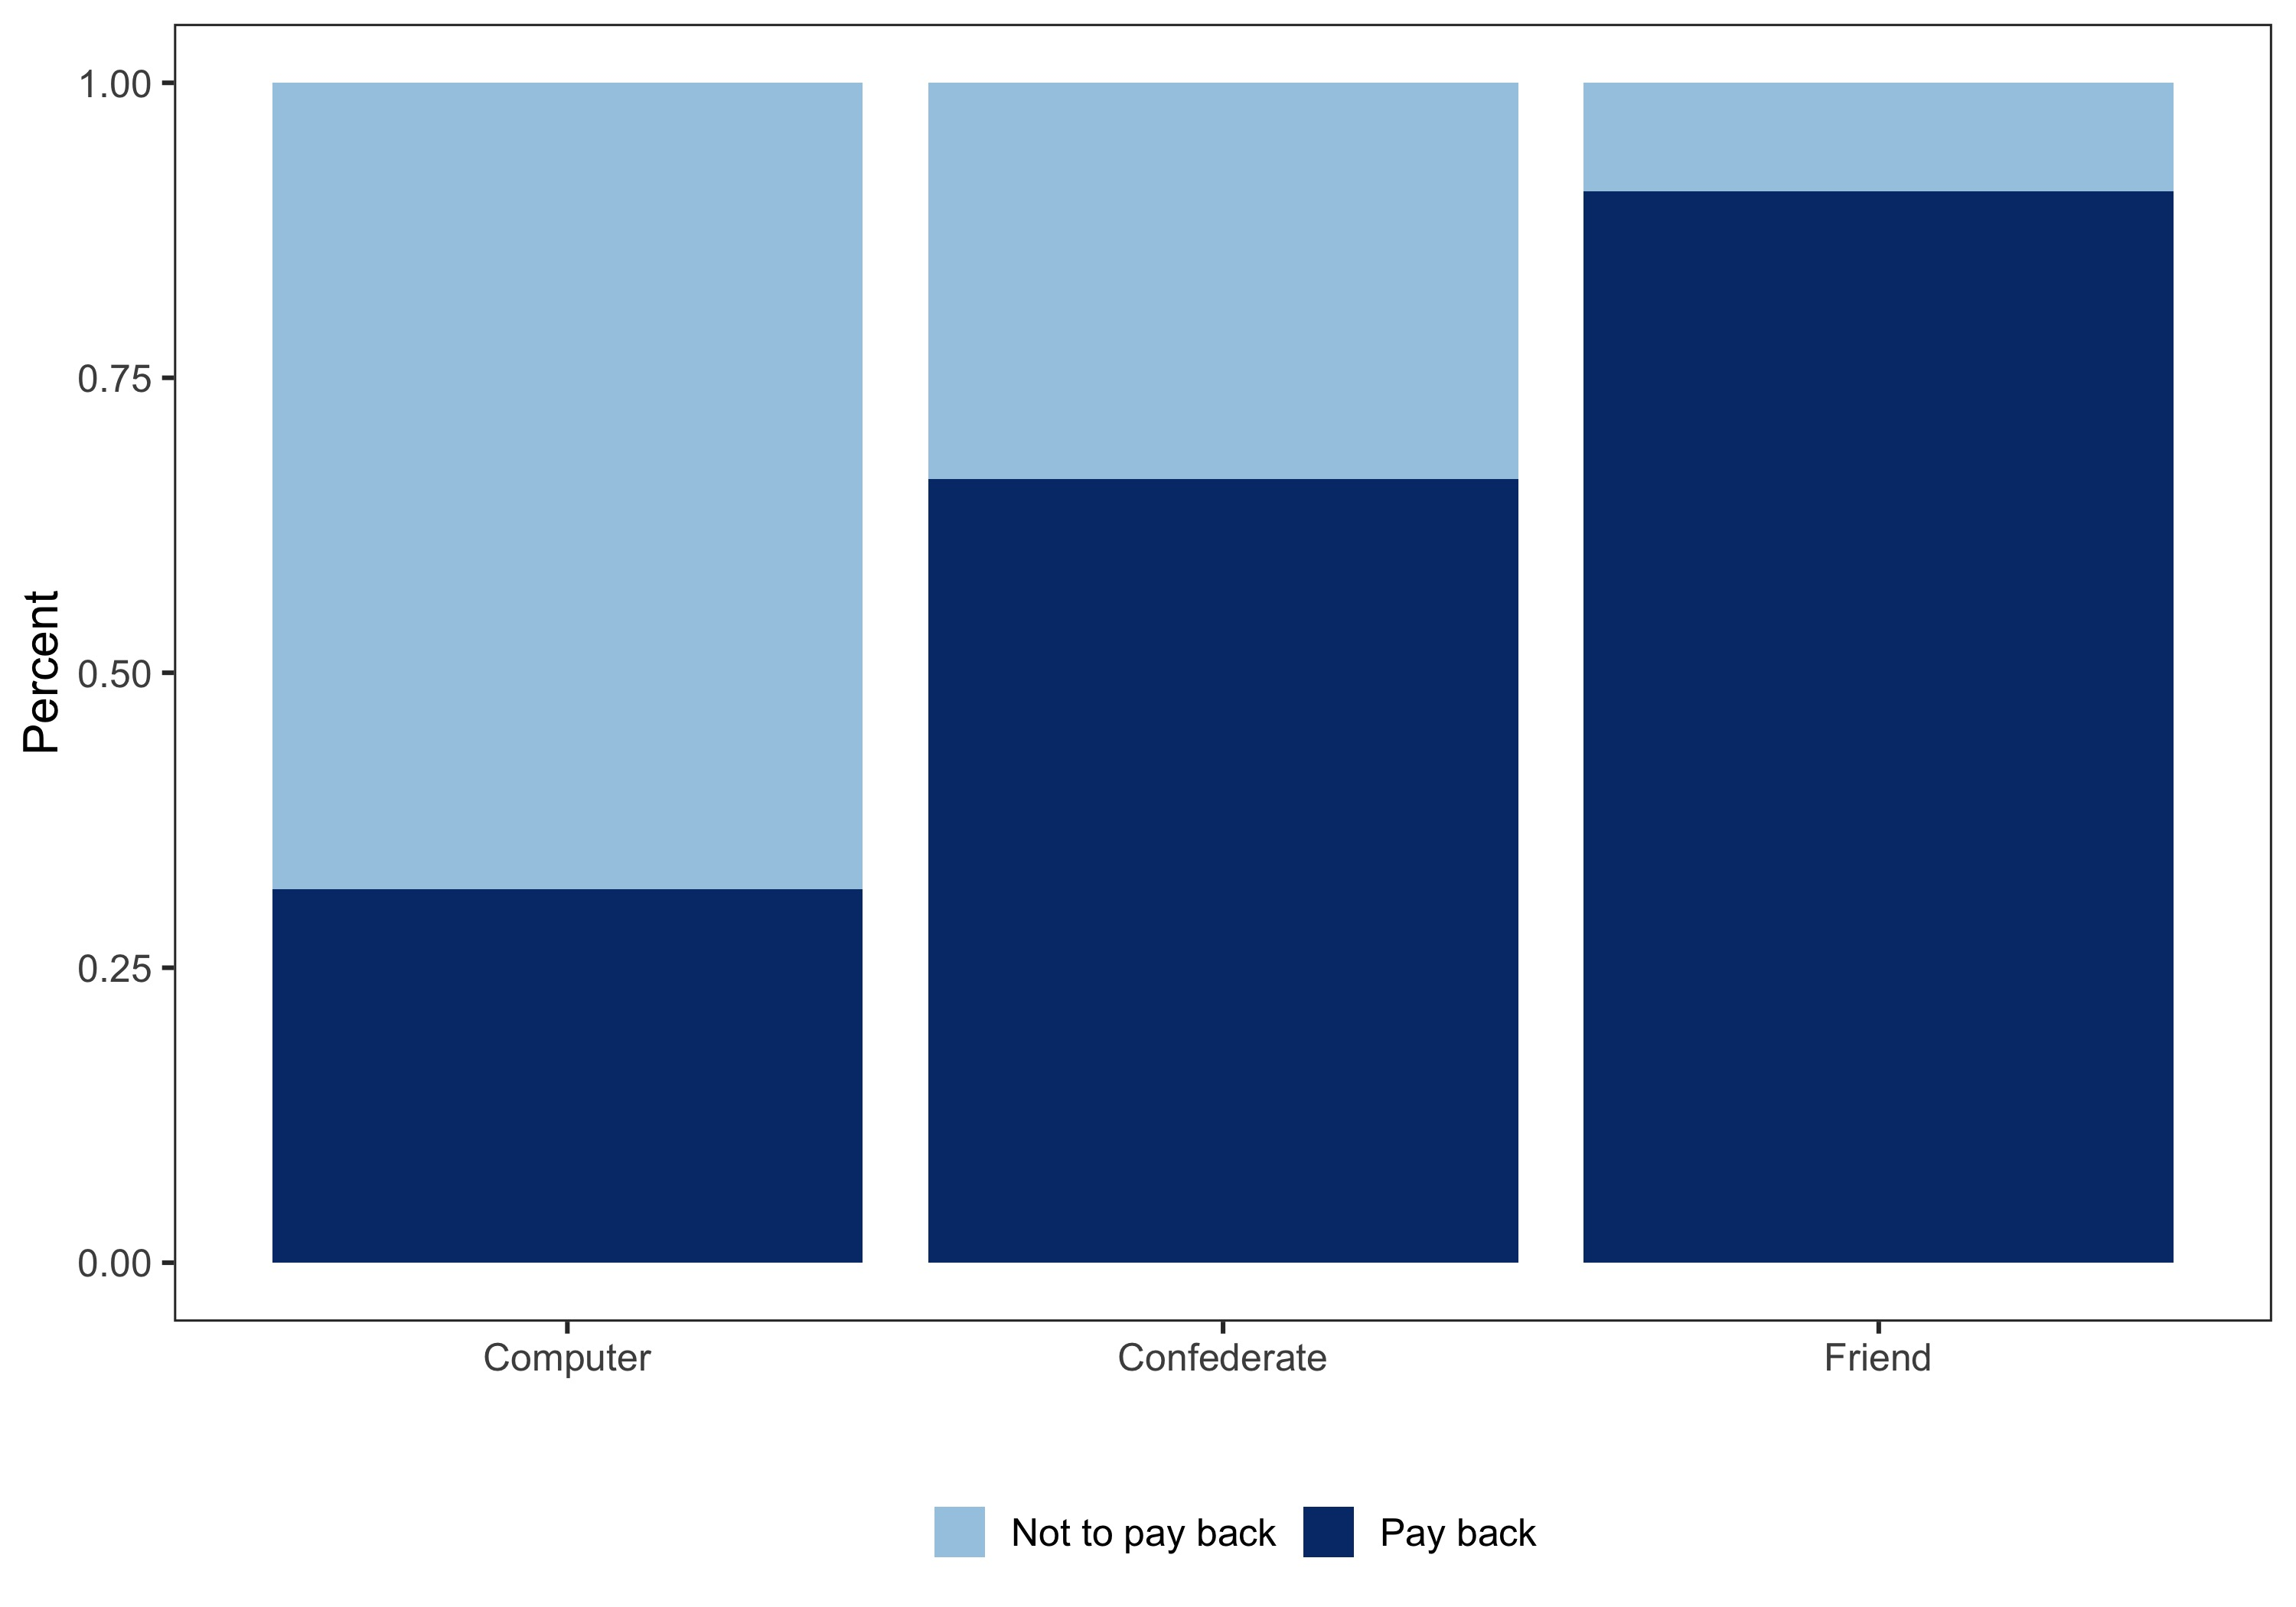
\includegraphics[width=0.8\linewidth]{/Users/saidjimenez/Documents/R/github_Said/social_closeness/Manuscript/figures/g2} 

}

\caption{Rates by partner}\label{fig:g2}
\end{figure}

\begin{figure}

{\centering 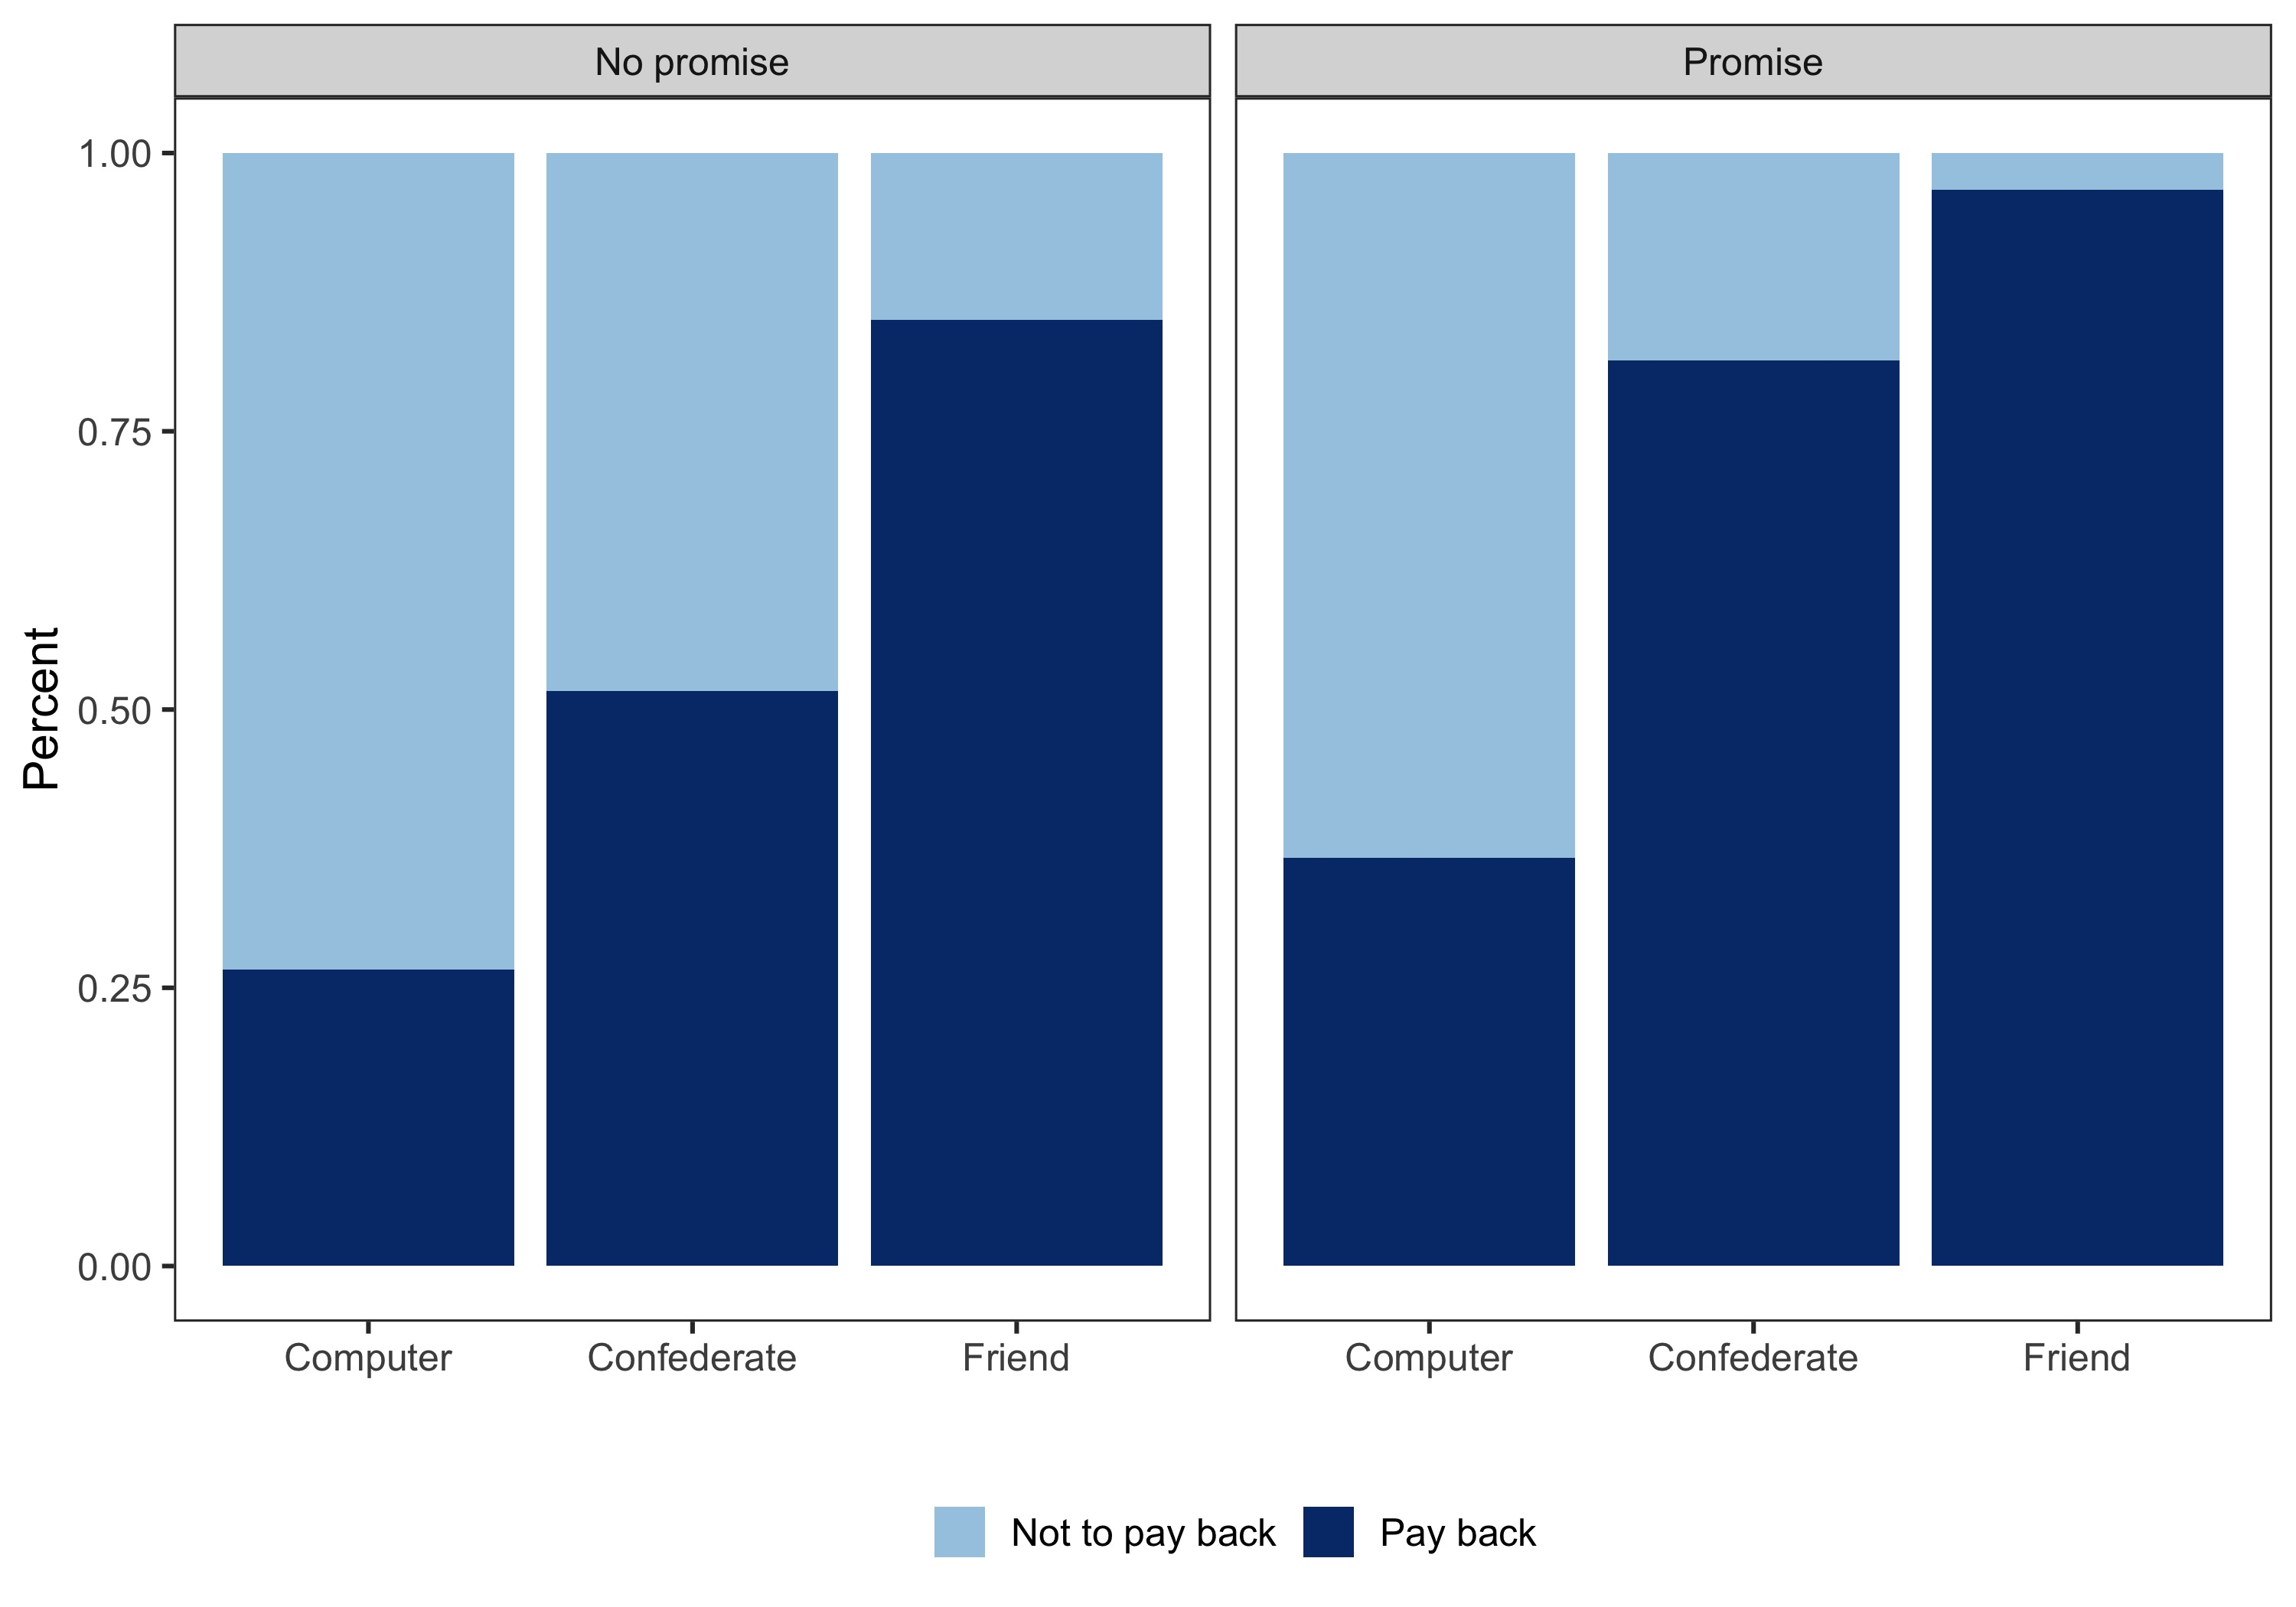
\includegraphics[width=0.8\linewidth]{/Users/saidjimenez/Documents/R/github_Said/social_closeness/Manuscript/figures/g3} 

}

\caption{Rates by partners and promise condition}\label{fig:g3}
\end{figure}

\begin{figure}

{\centering 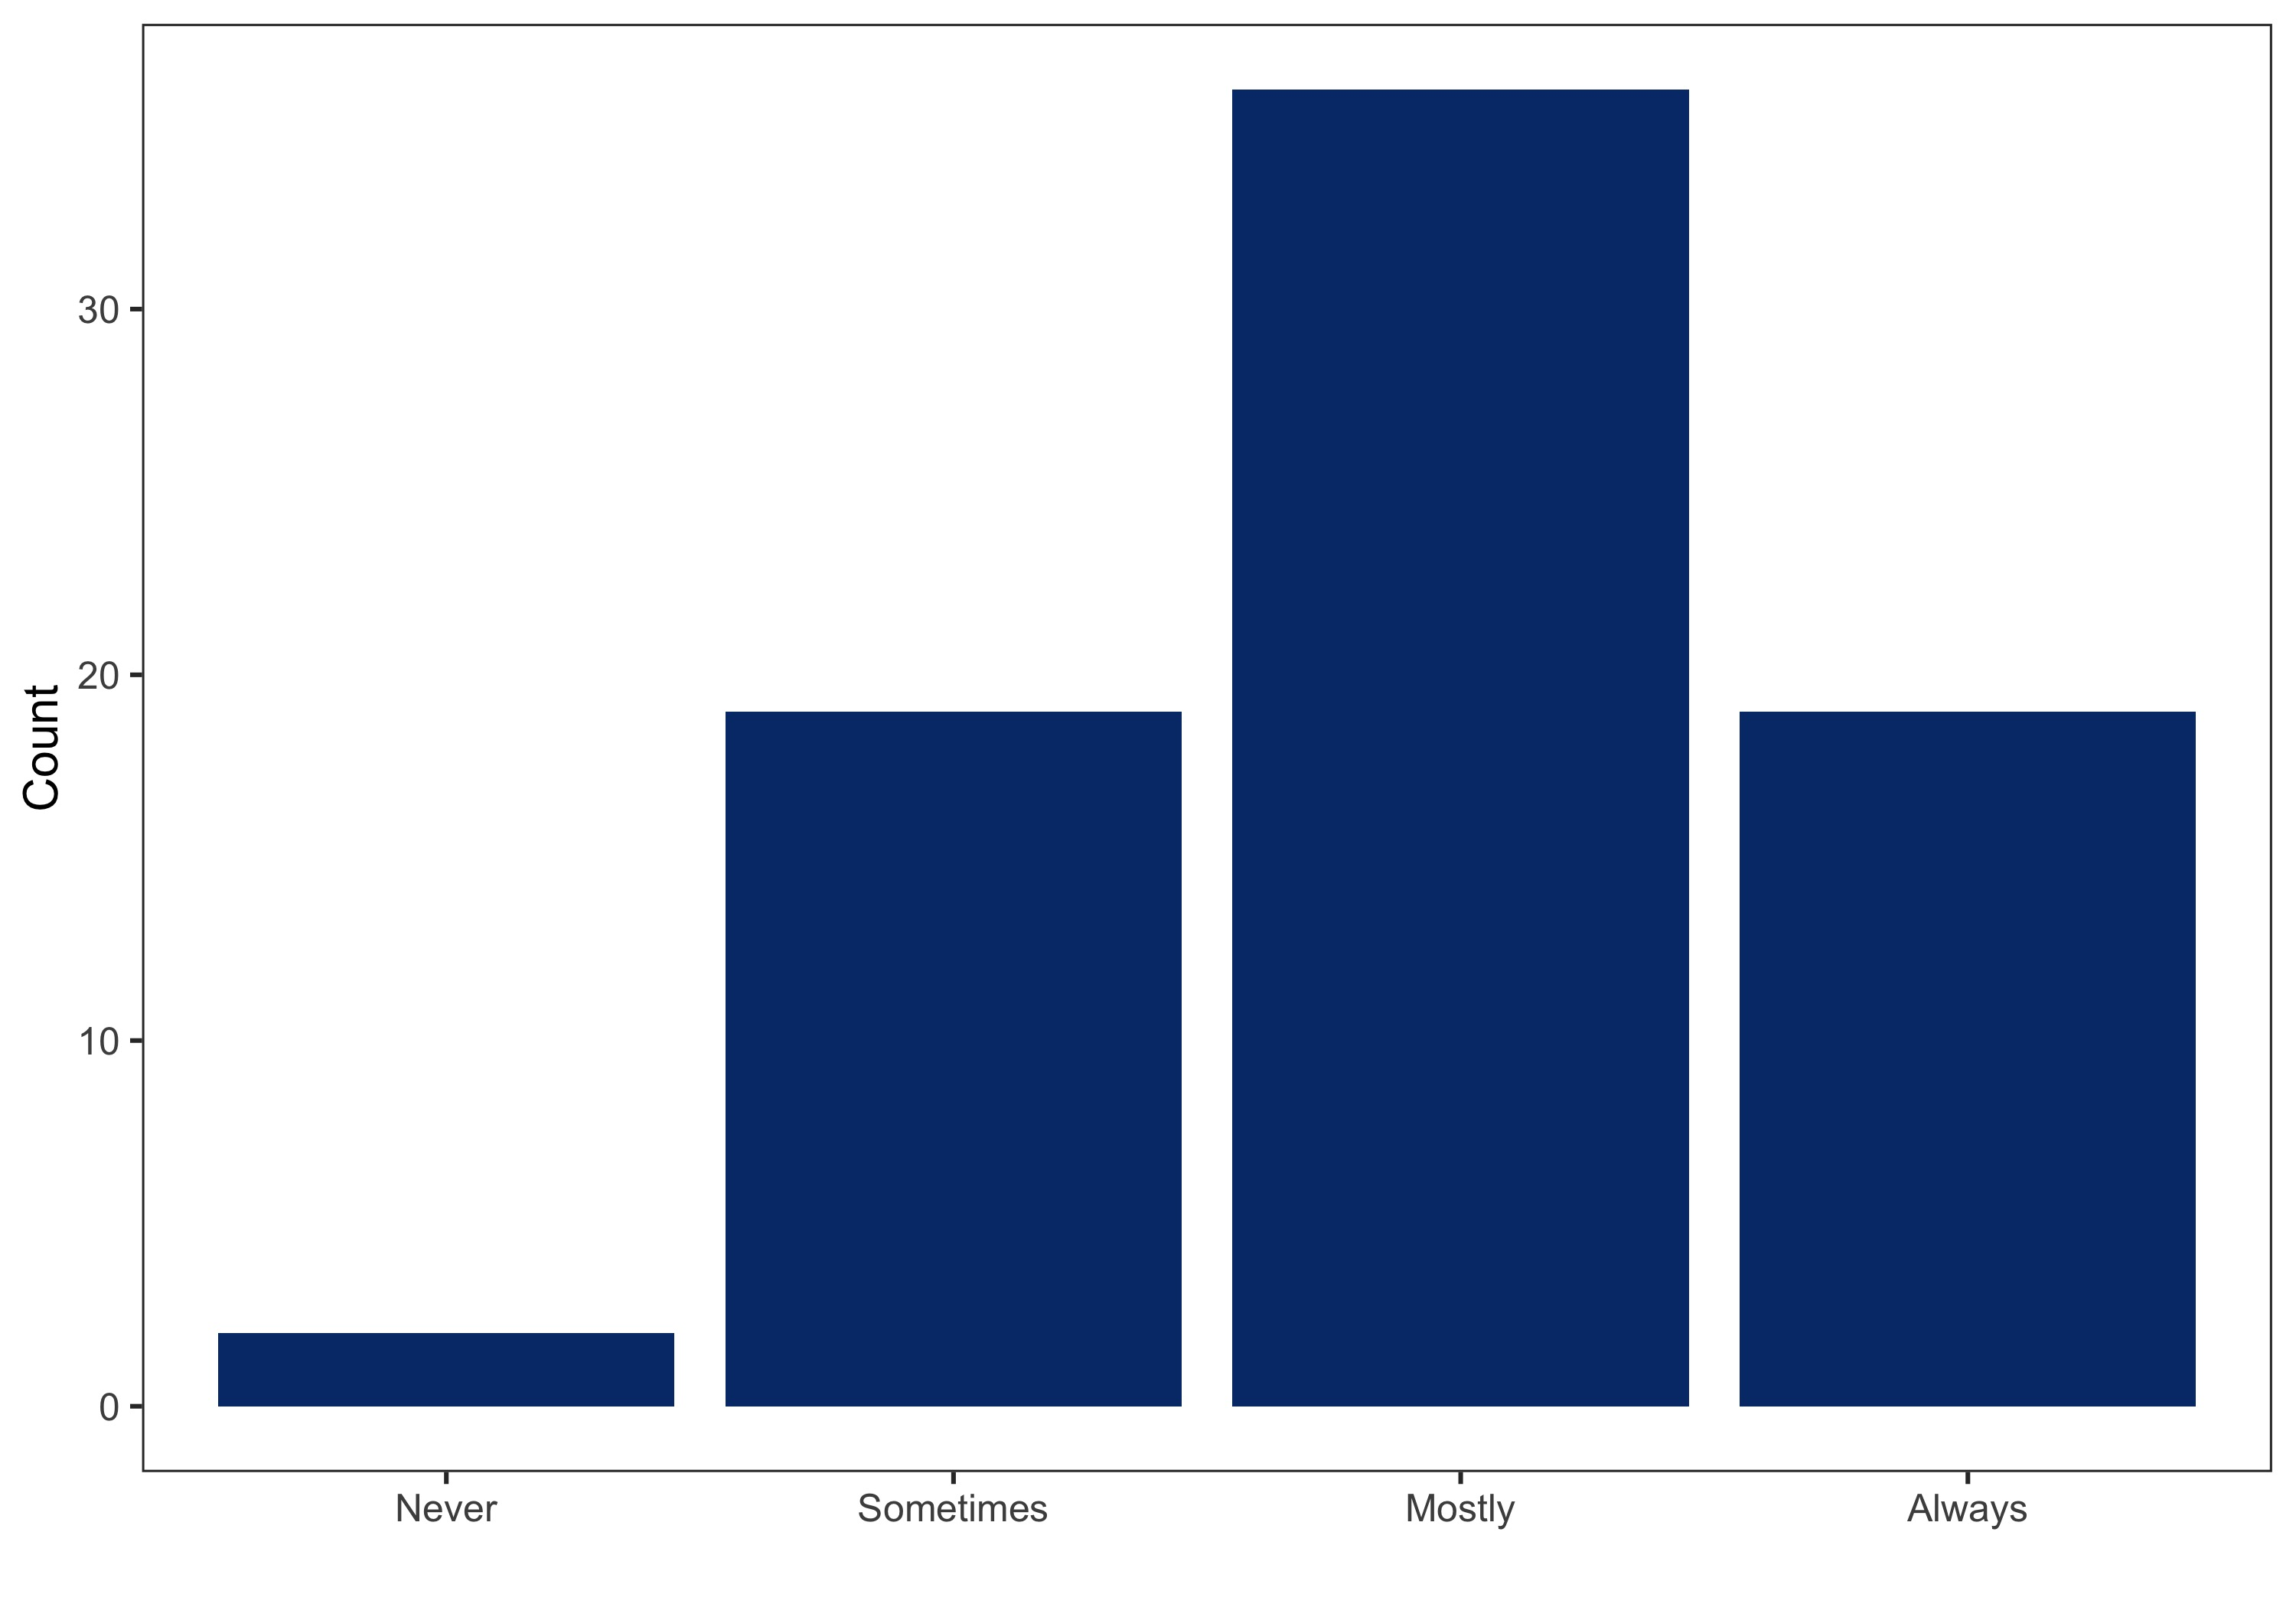
\includegraphics[width=0.8\linewidth]{/Users/saidjimenez/Documents/R/github_Said/social_closeness/Manuscript/figures/g4} 

}

\caption{Promises}\label{fig:g4}
\end{figure}

\begin{figure}

{\centering 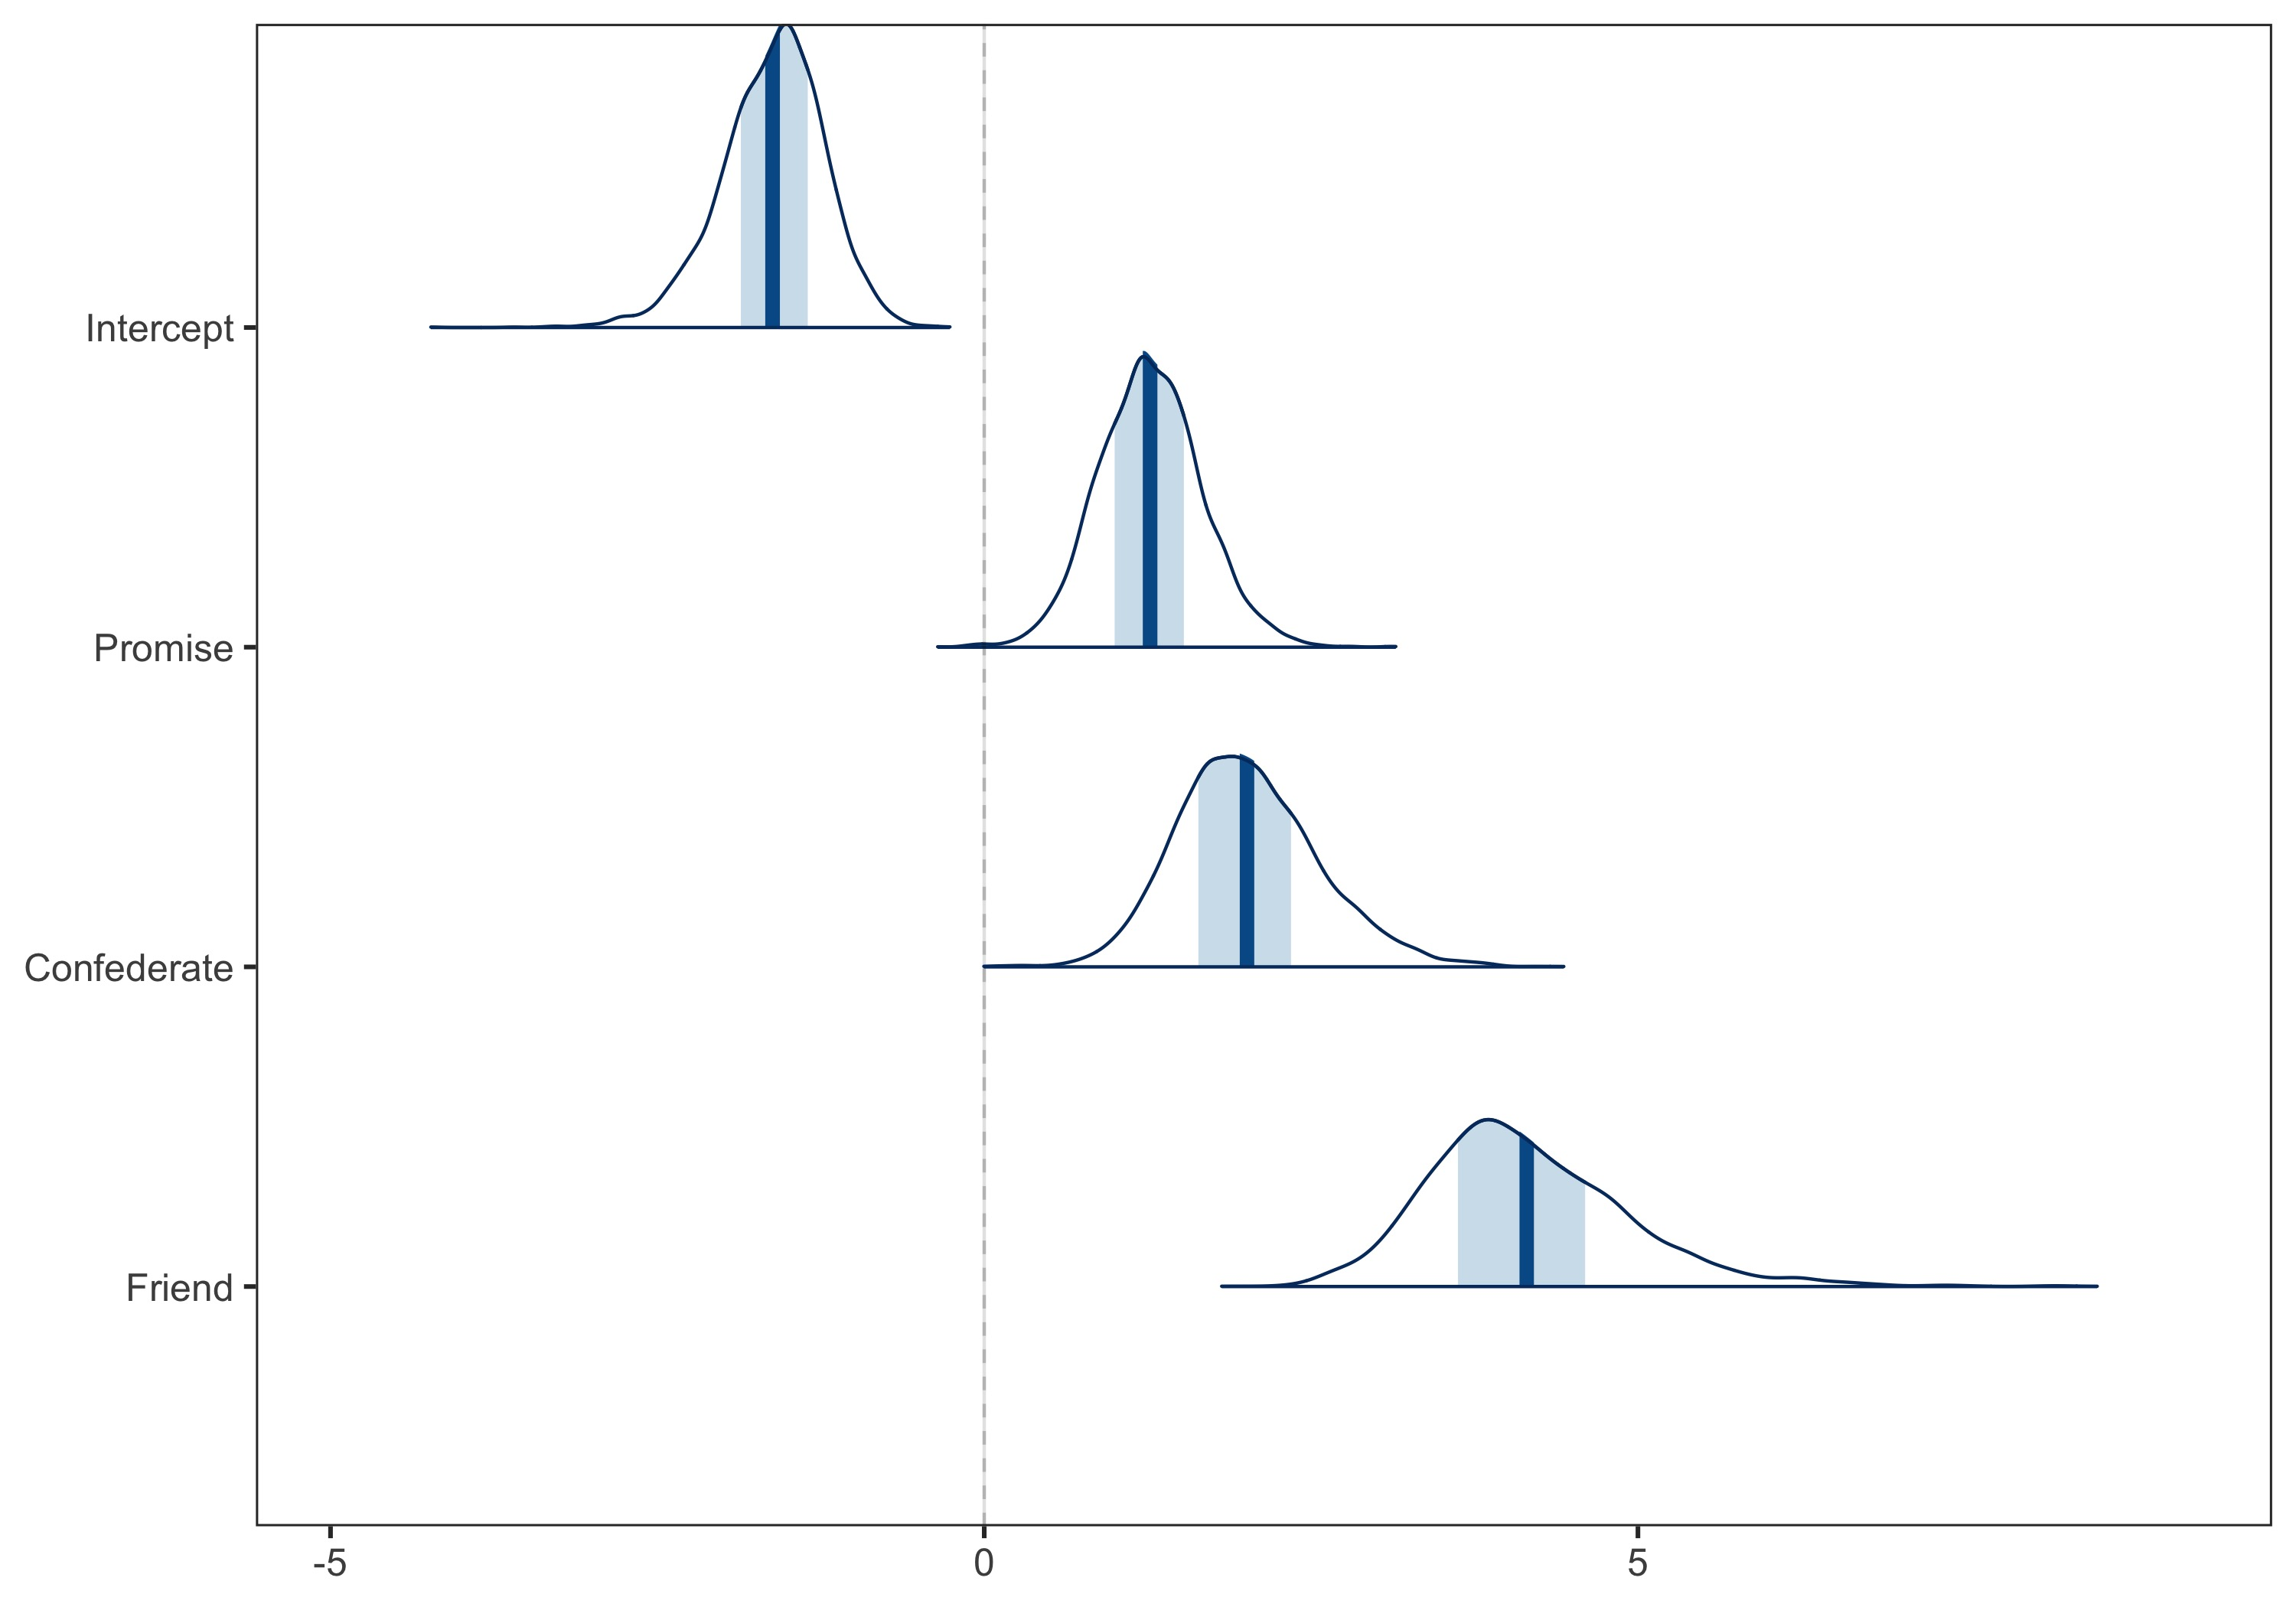
\includegraphics[width=0.8\linewidth]{/Users/saidjimenez/Documents/R/github_Said/social_closeness/Manuscript/figures/g5} 

}

\caption{Bayesians logistic coefficients}\label{fig:g5}
\end{figure}

\begin{figure}

{\centering 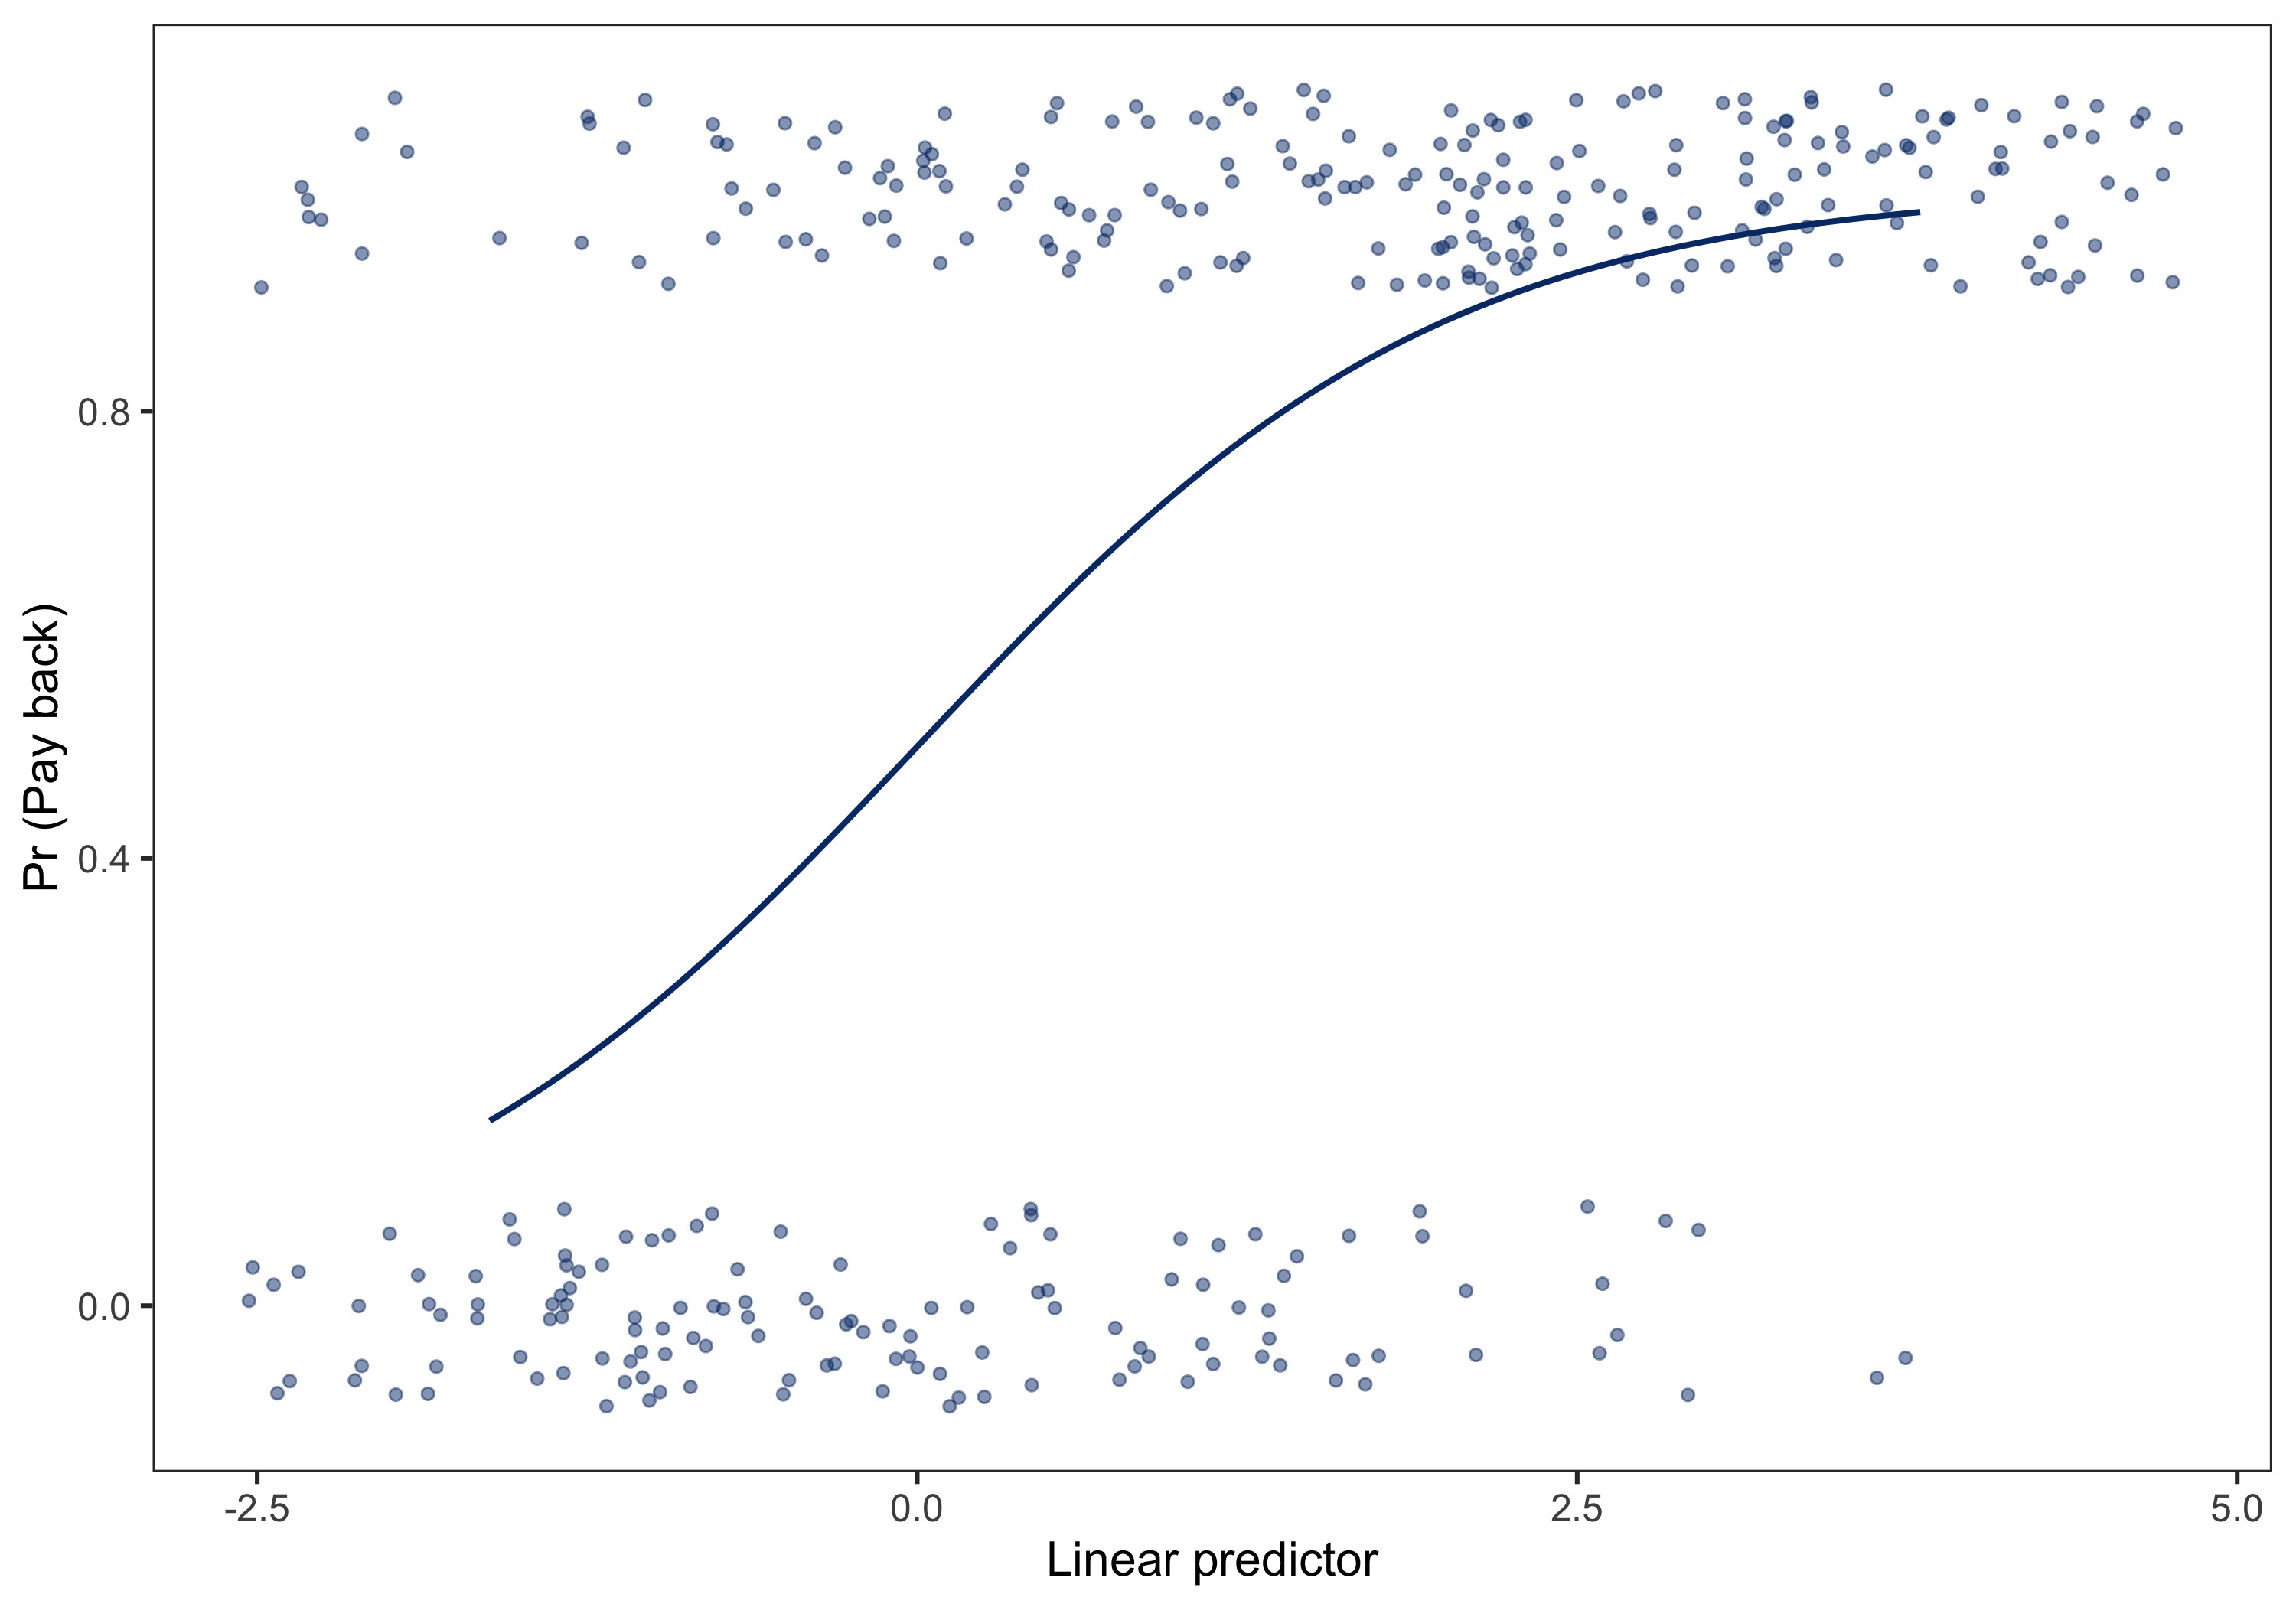
\includegraphics[width=0.8\linewidth]{/Users/saidjimenez/Documents/R/github_Said/social_closeness/Manuscript/figures/g6} 

}

\caption{Linear population predictor}\label{fig:g6}
\end{figure}

\begin{figure}

{\centering 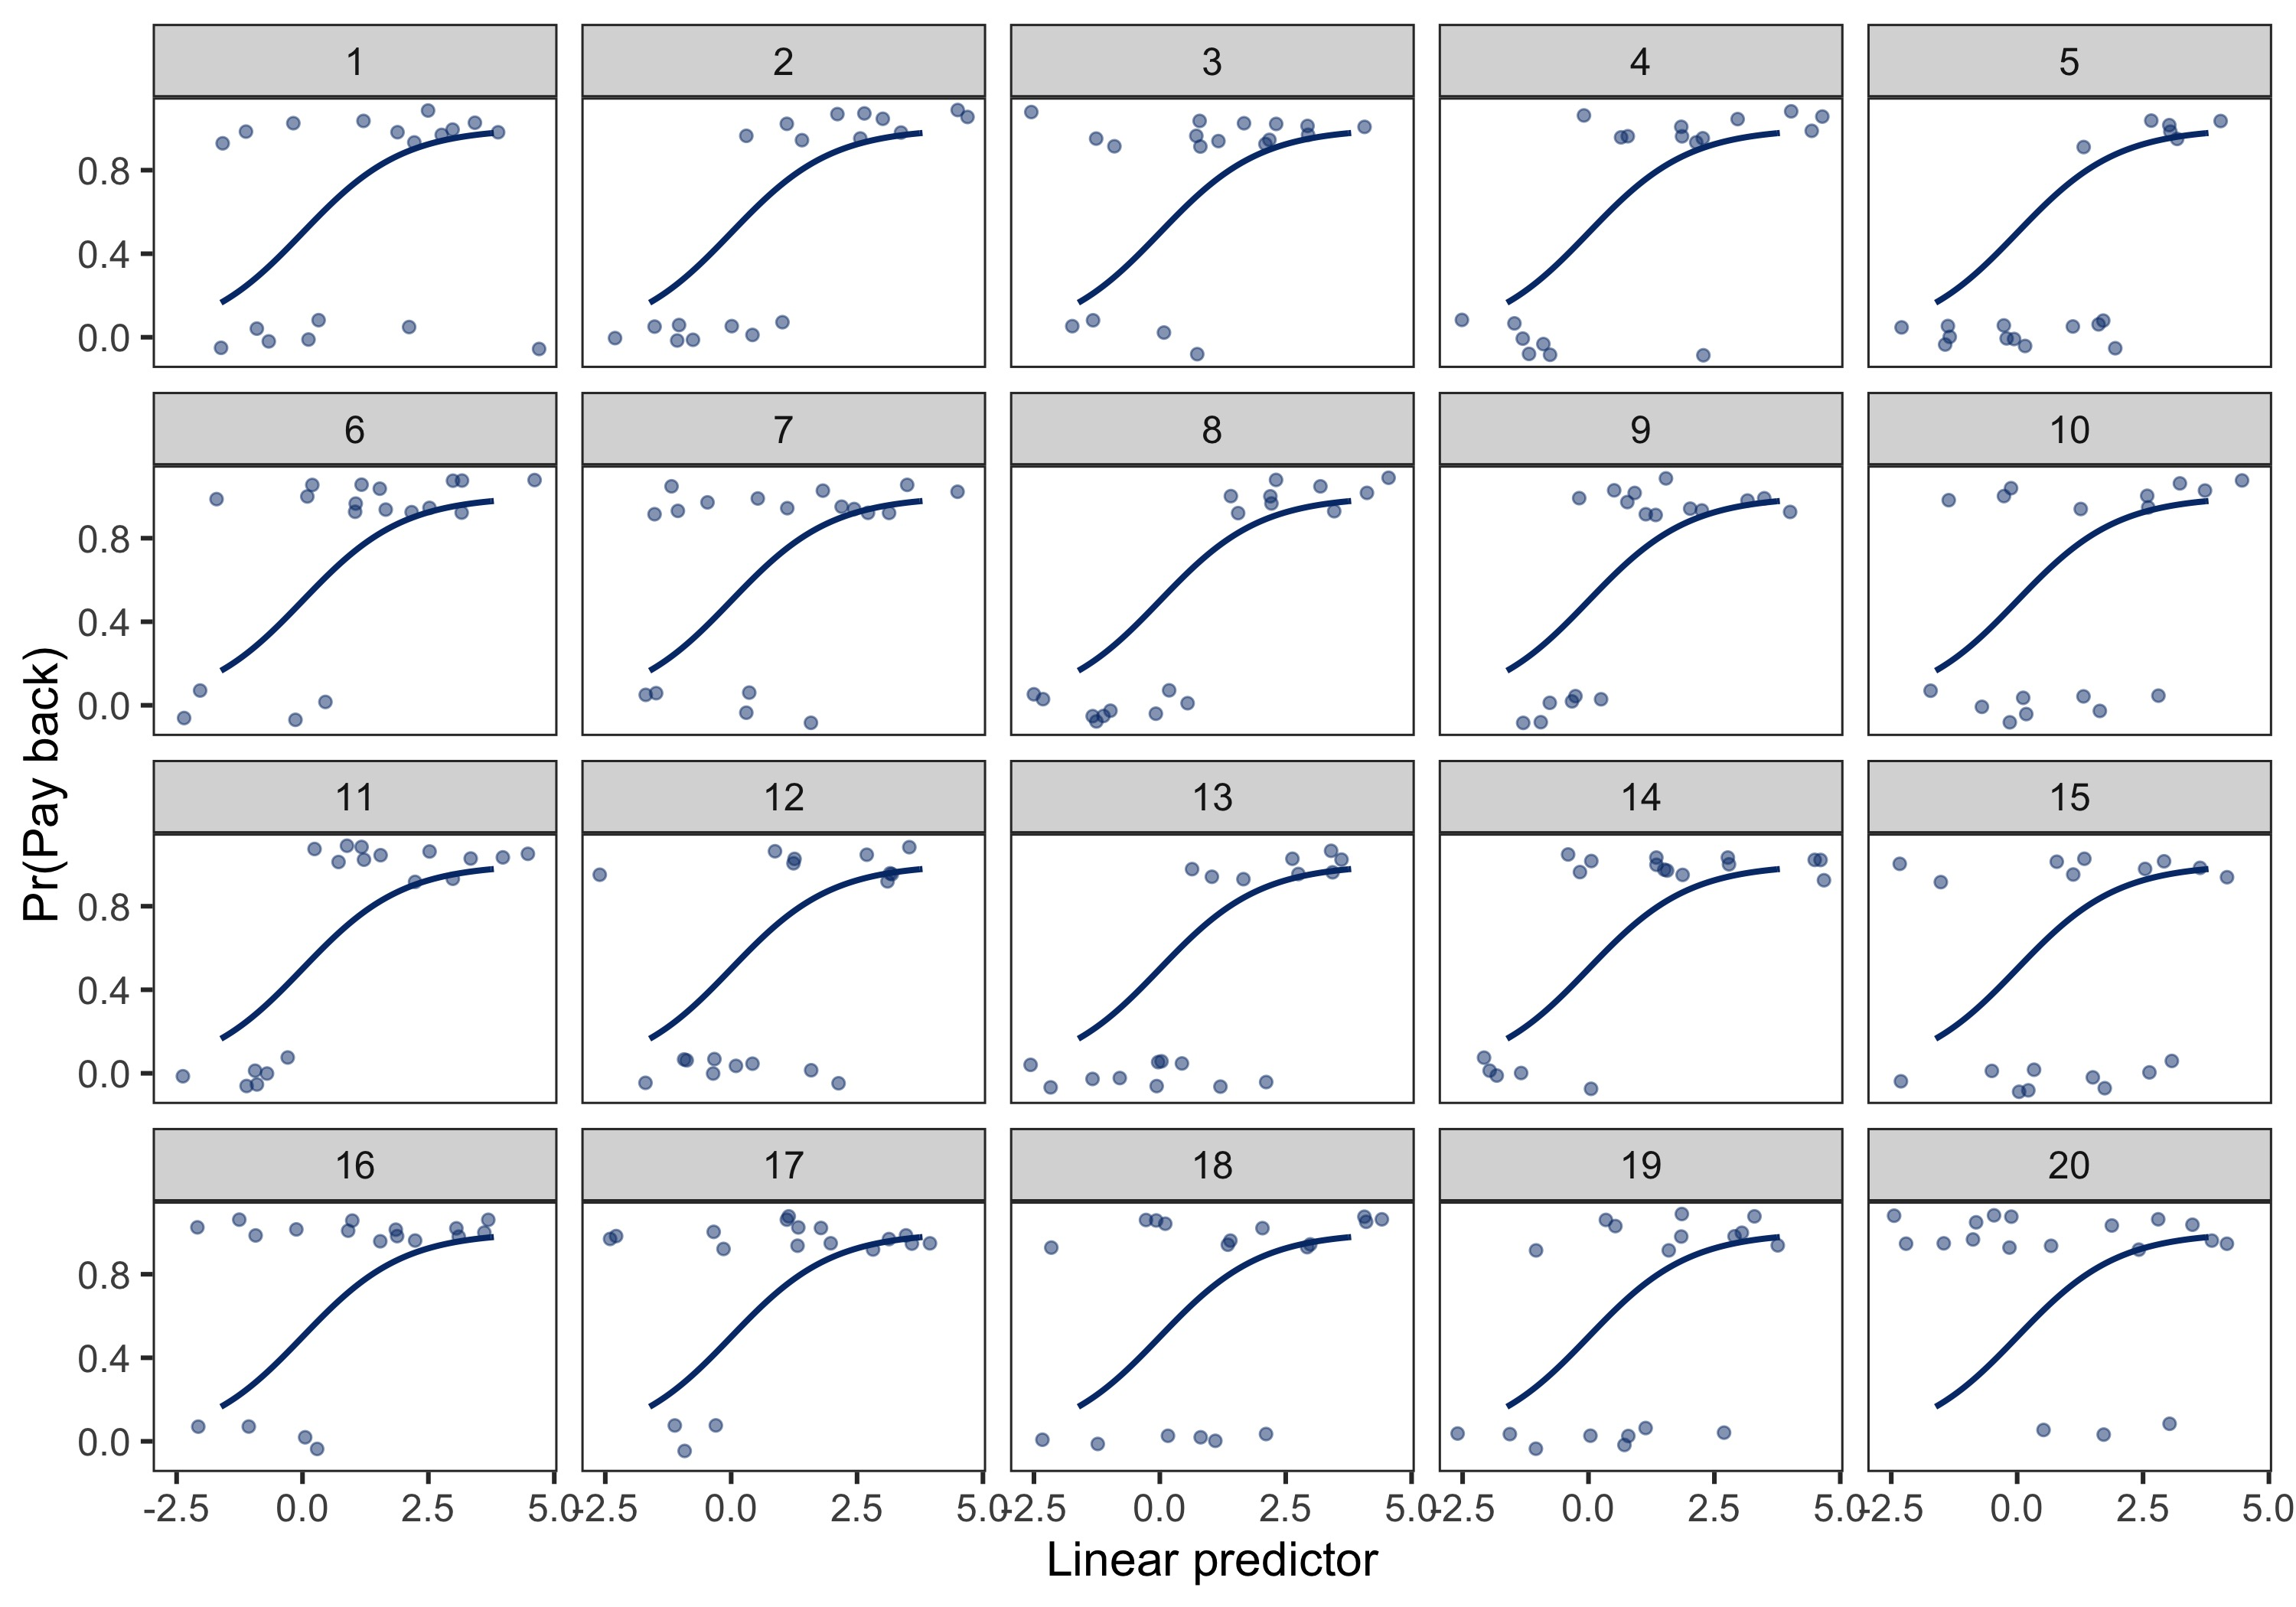
\includegraphics[width=0.8\linewidth]{/Users/saidjimenez/Documents/R/github_Said/social_closeness/Manuscript/figures/g7} 

}

\caption{Linear population predictor by subject}\label{fig:g7}
\end{figure}

\begin{figure}

{\centering 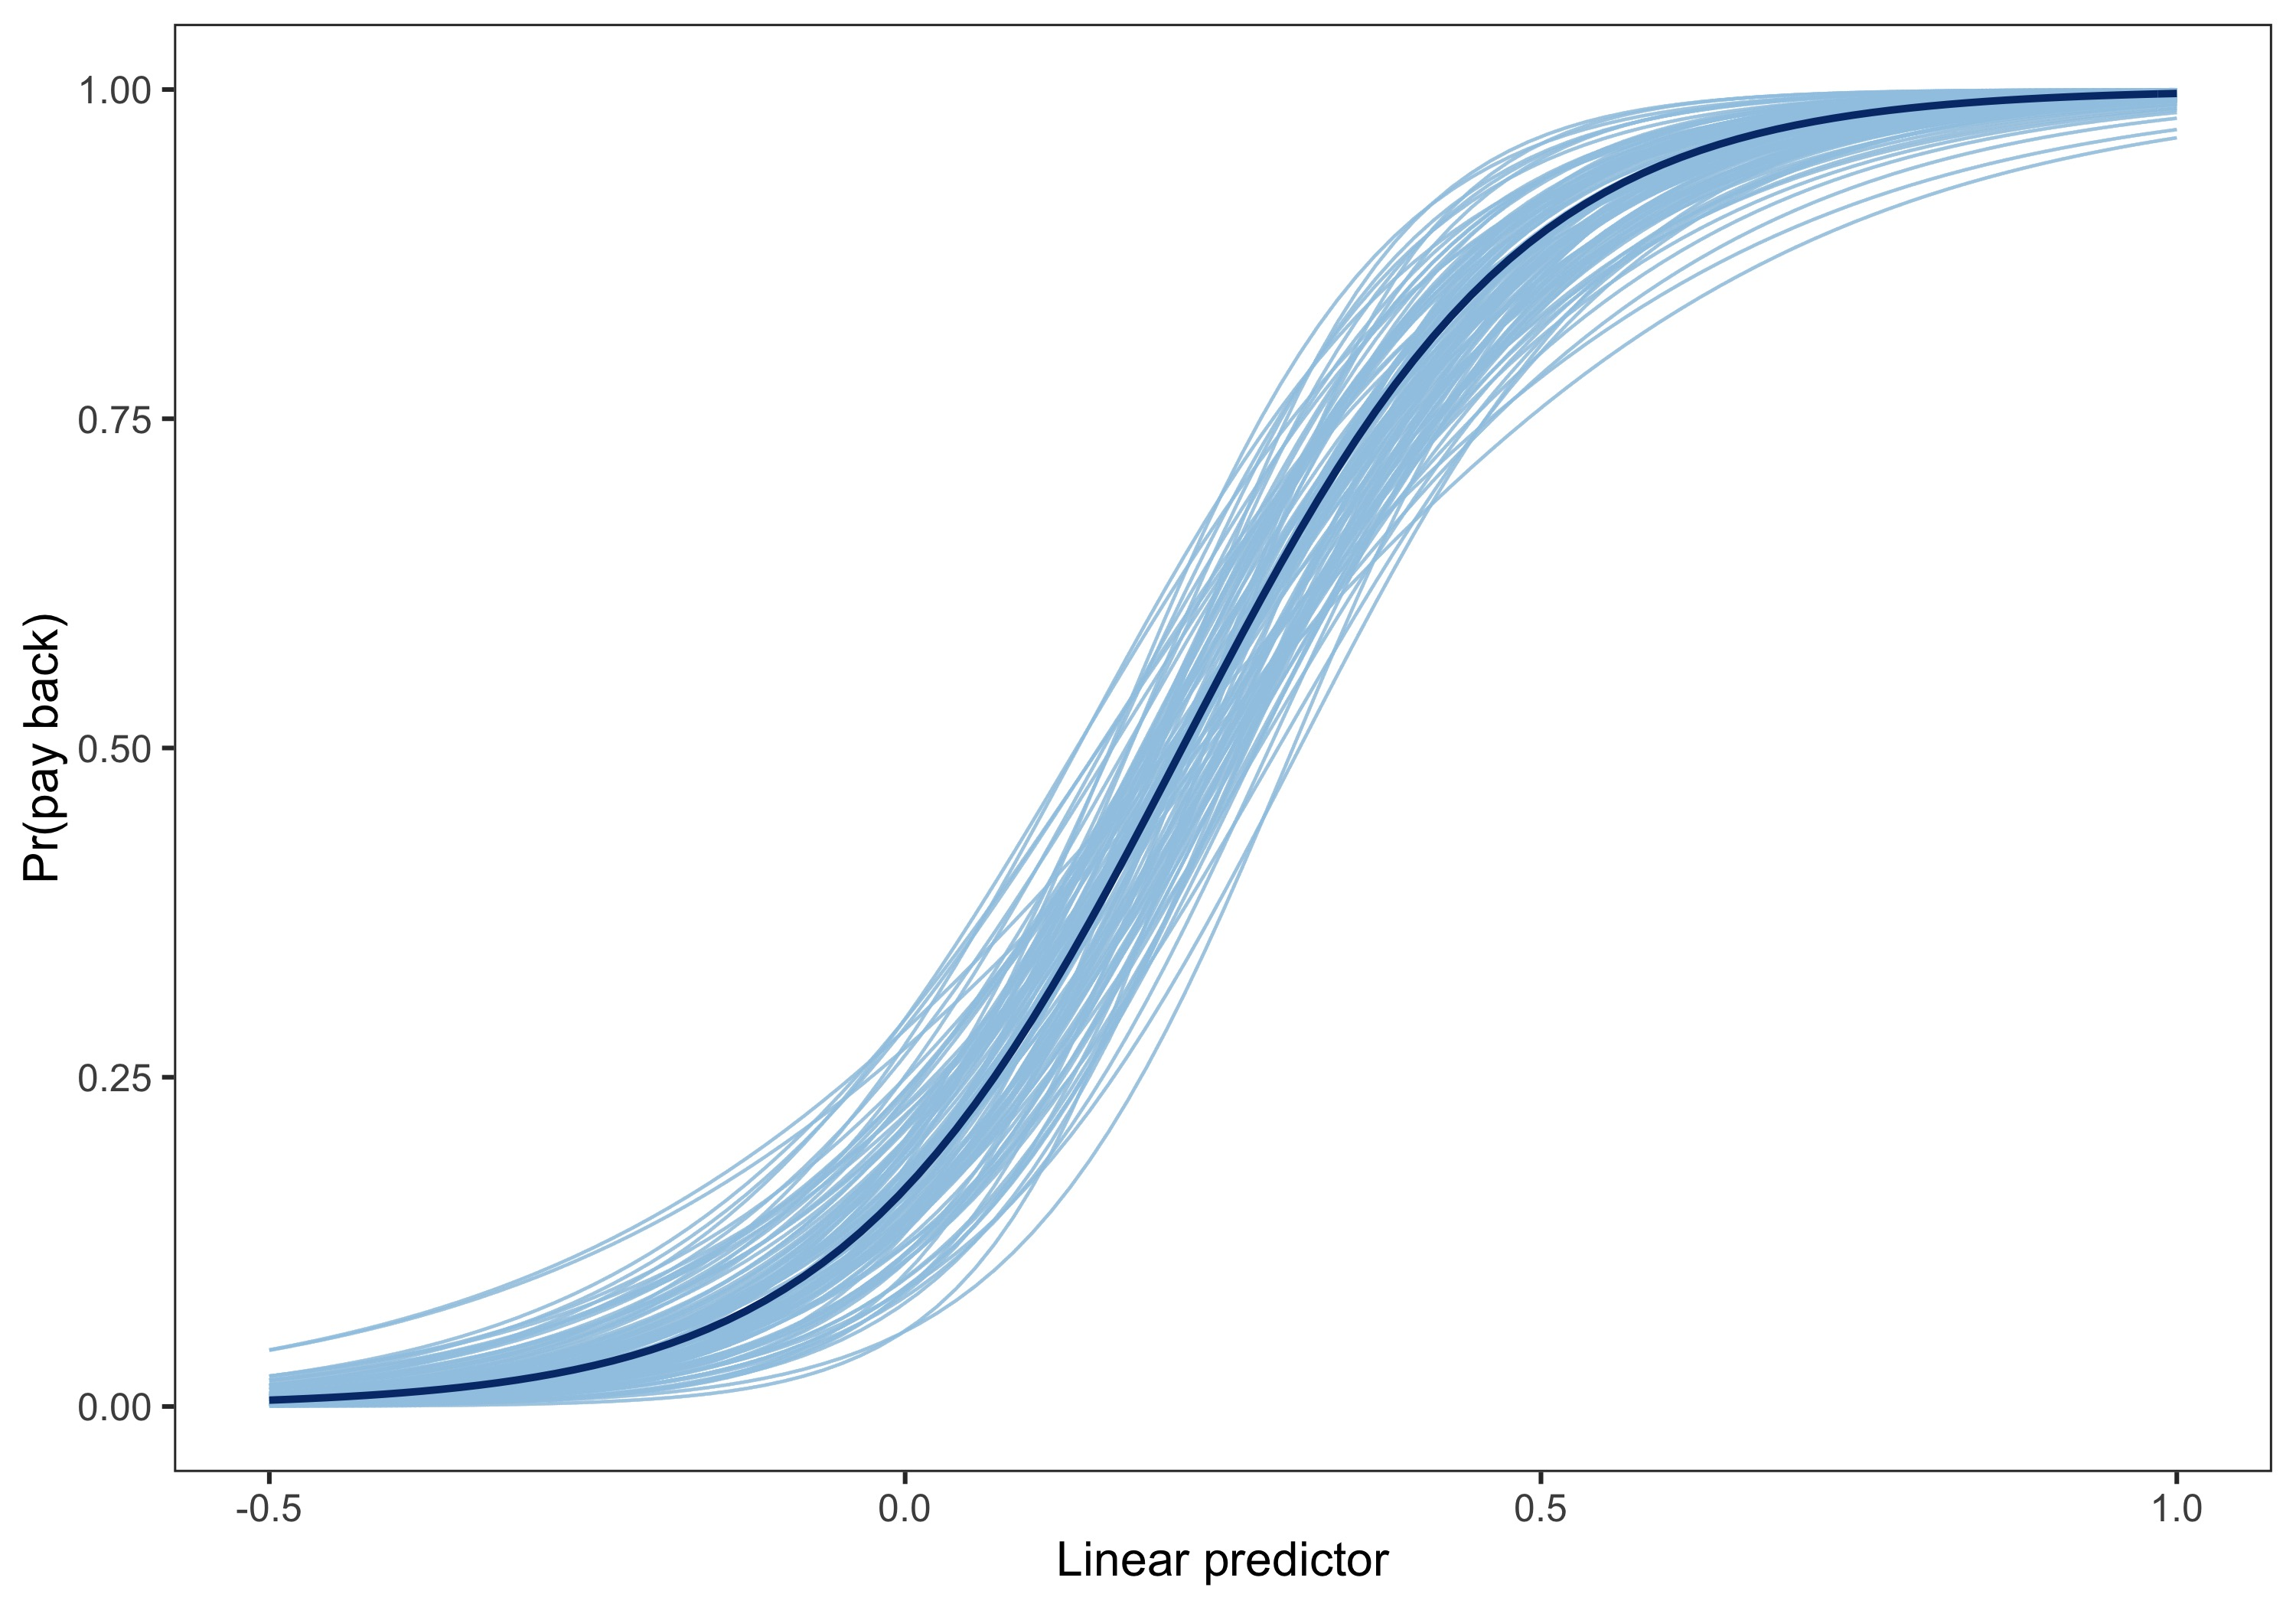
\includegraphics[width=0.8\linewidth]{/Users/saidjimenez/Documents/R/github_Said/social_closeness/Manuscript/figures/g8} 

}

\caption{Population coefficient with uncertainty}\label{fig:g8}
\end{figure}

\begin{figure}

{\centering 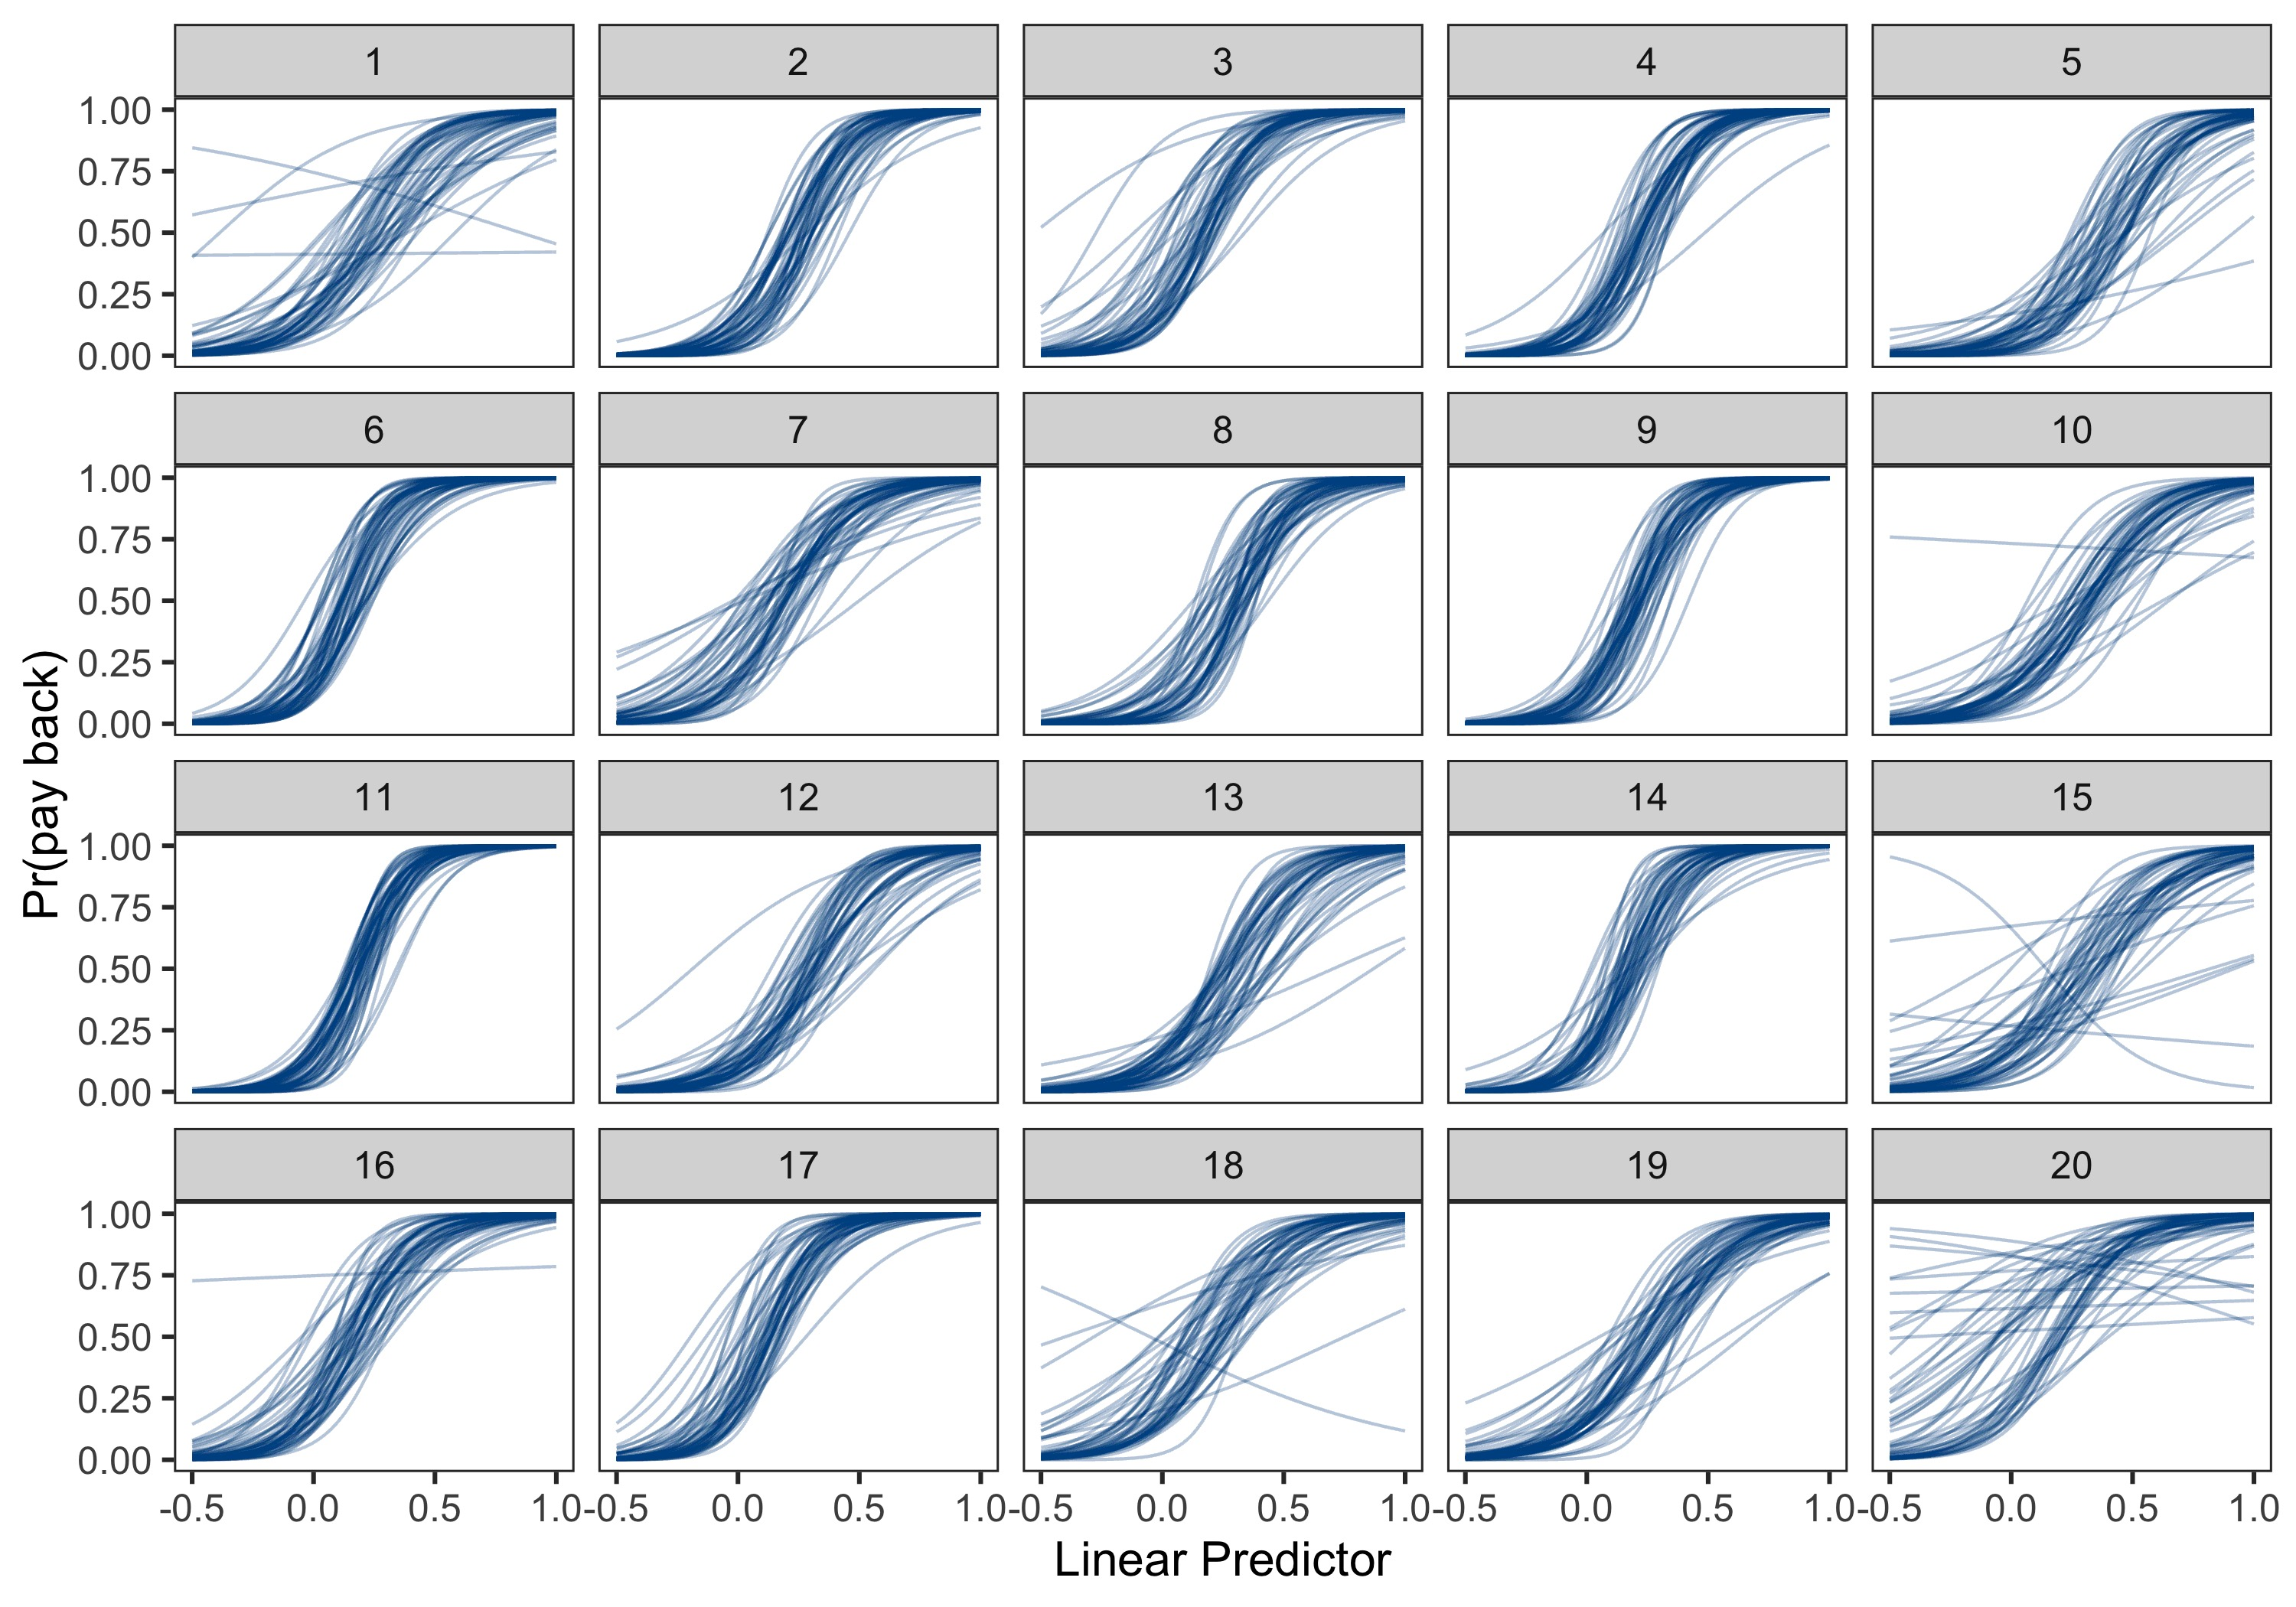
\includegraphics[width=0.8\linewidth]{/Users/saidjimenez/Documents/R/github_Said/social_closeness/Manuscript/figures/g9} 

}

\caption{Model adjusted by subject}\label{fig:g9}
\end{figure}

\begin{figure}

{\centering 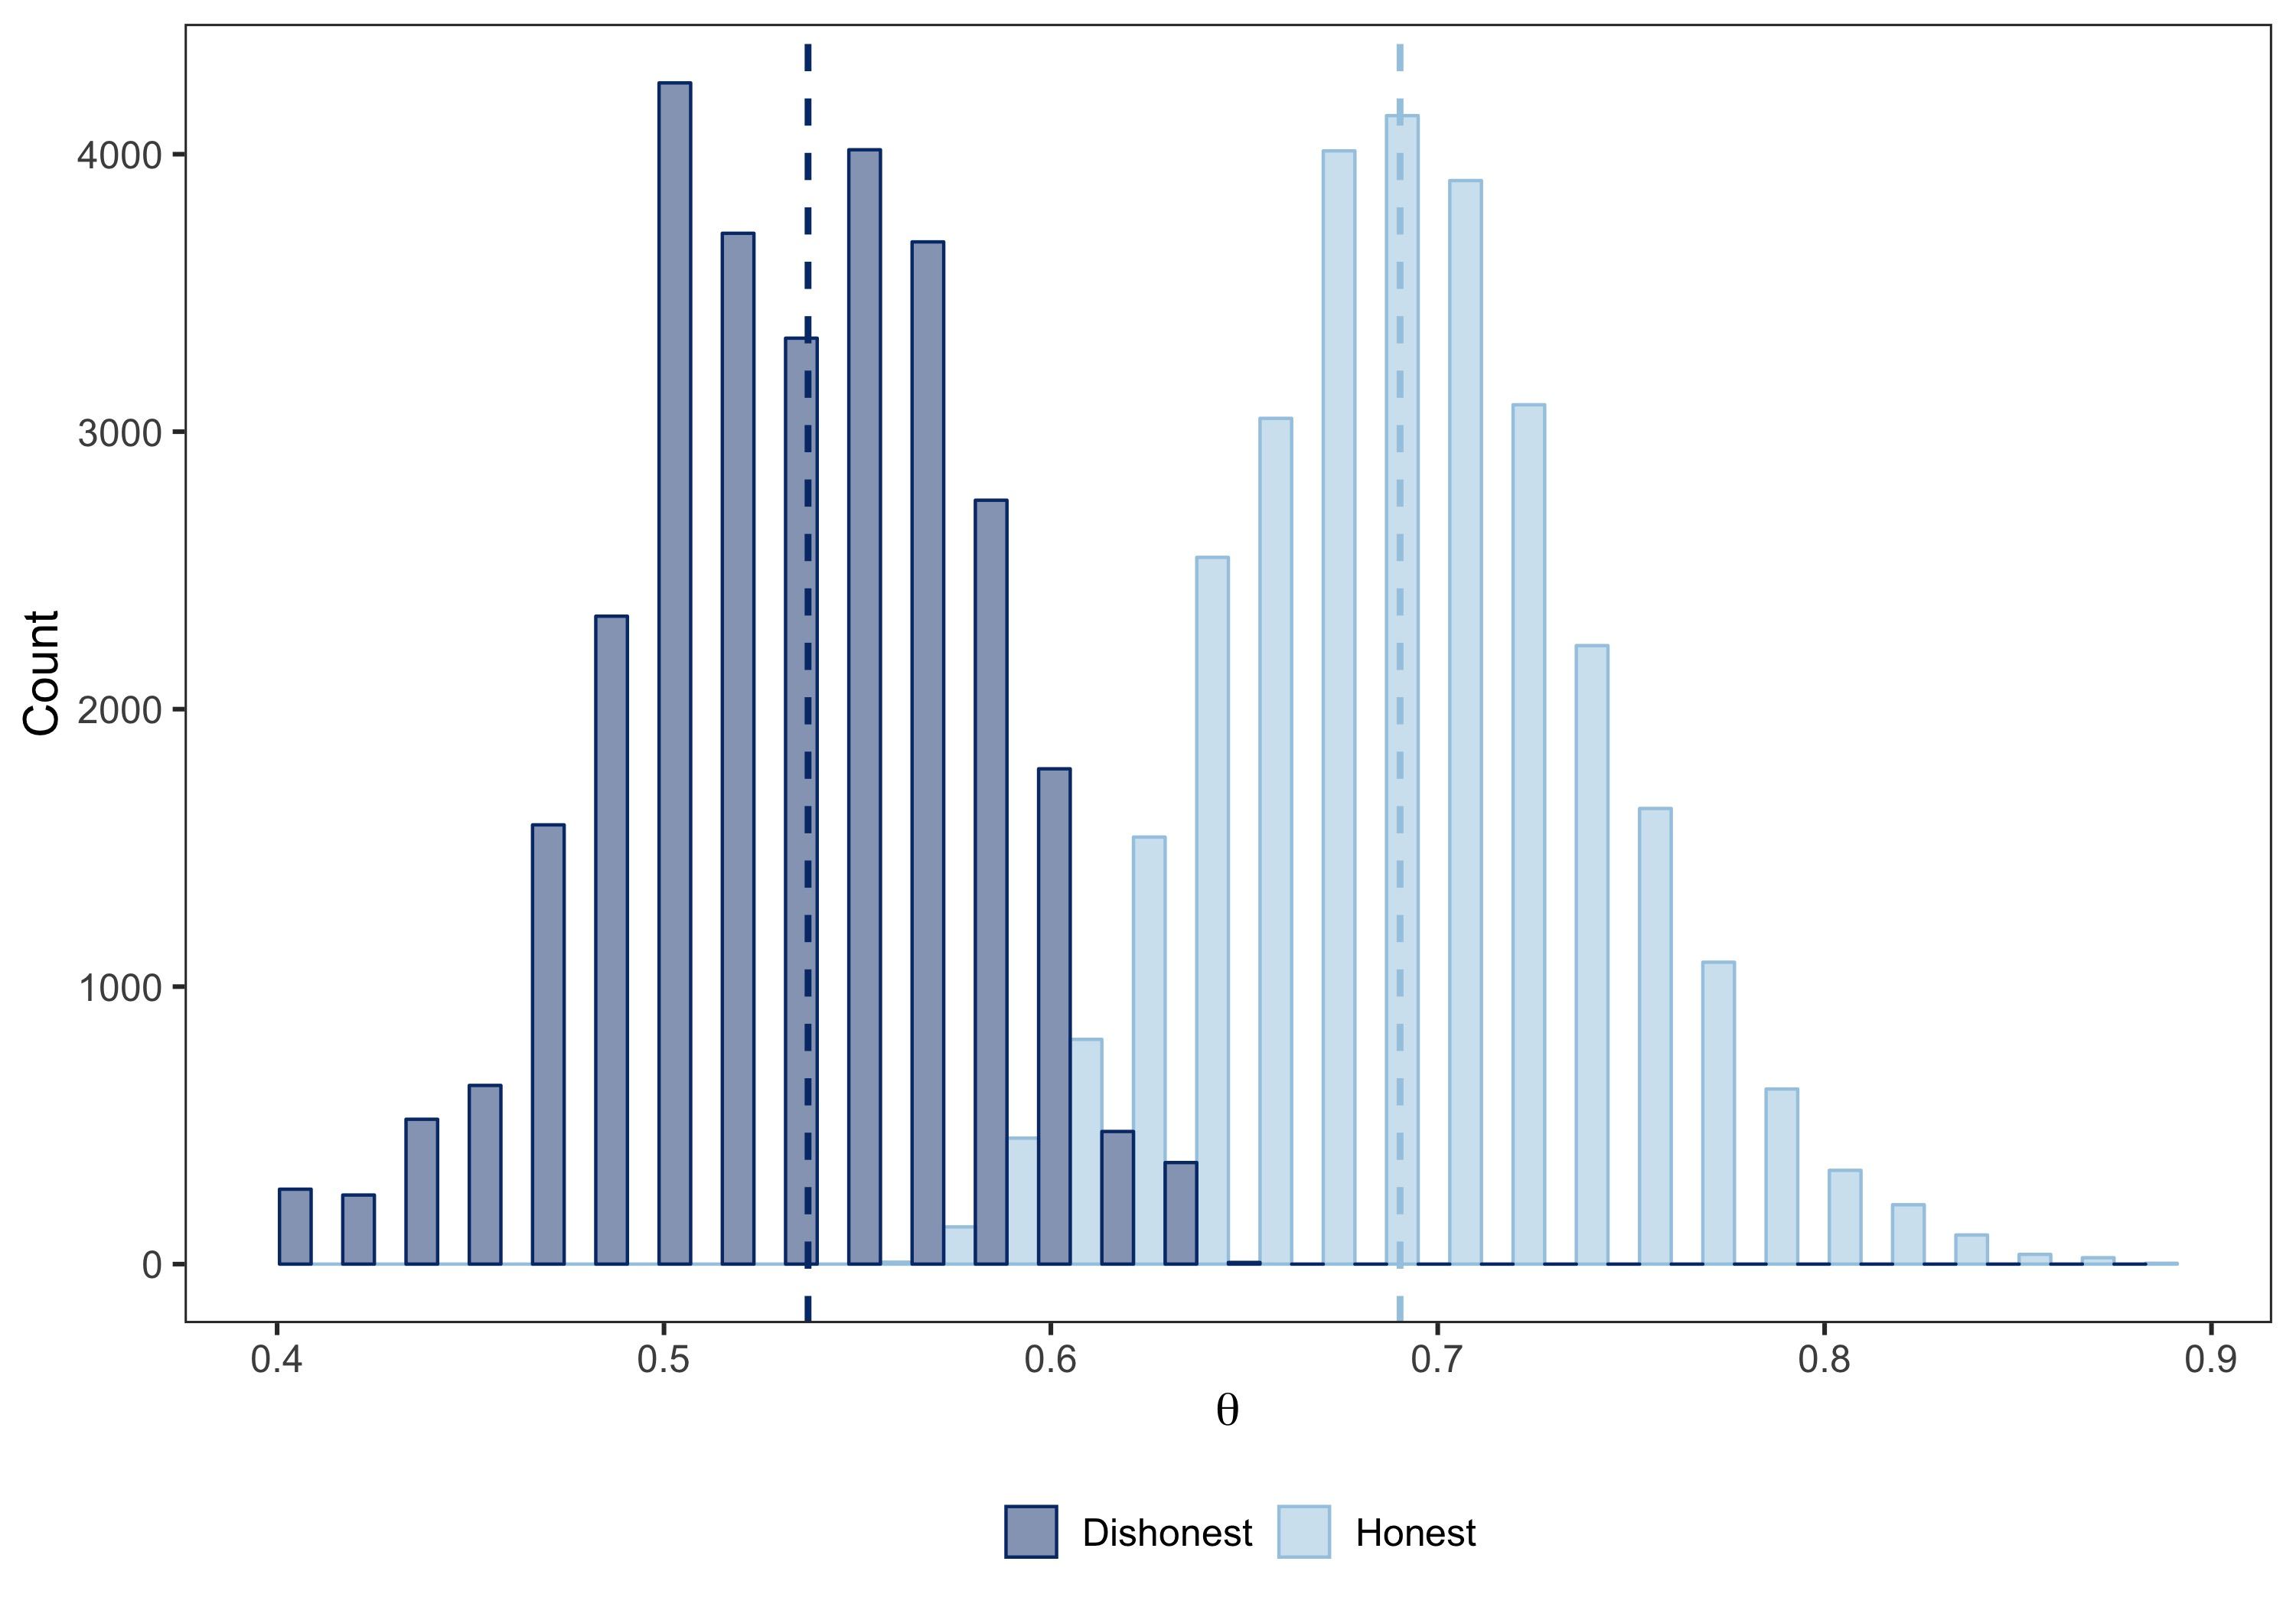
\includegraphics[width=0.8\linewidth]{/Users/saidjimenez/Documents/R/github_Said/social_closeness/Manuscript/figures/g16} 

}

\caption{Two latent thetas}\label{fig:g16}
\end{figure}

\begin{figure}

{\centering 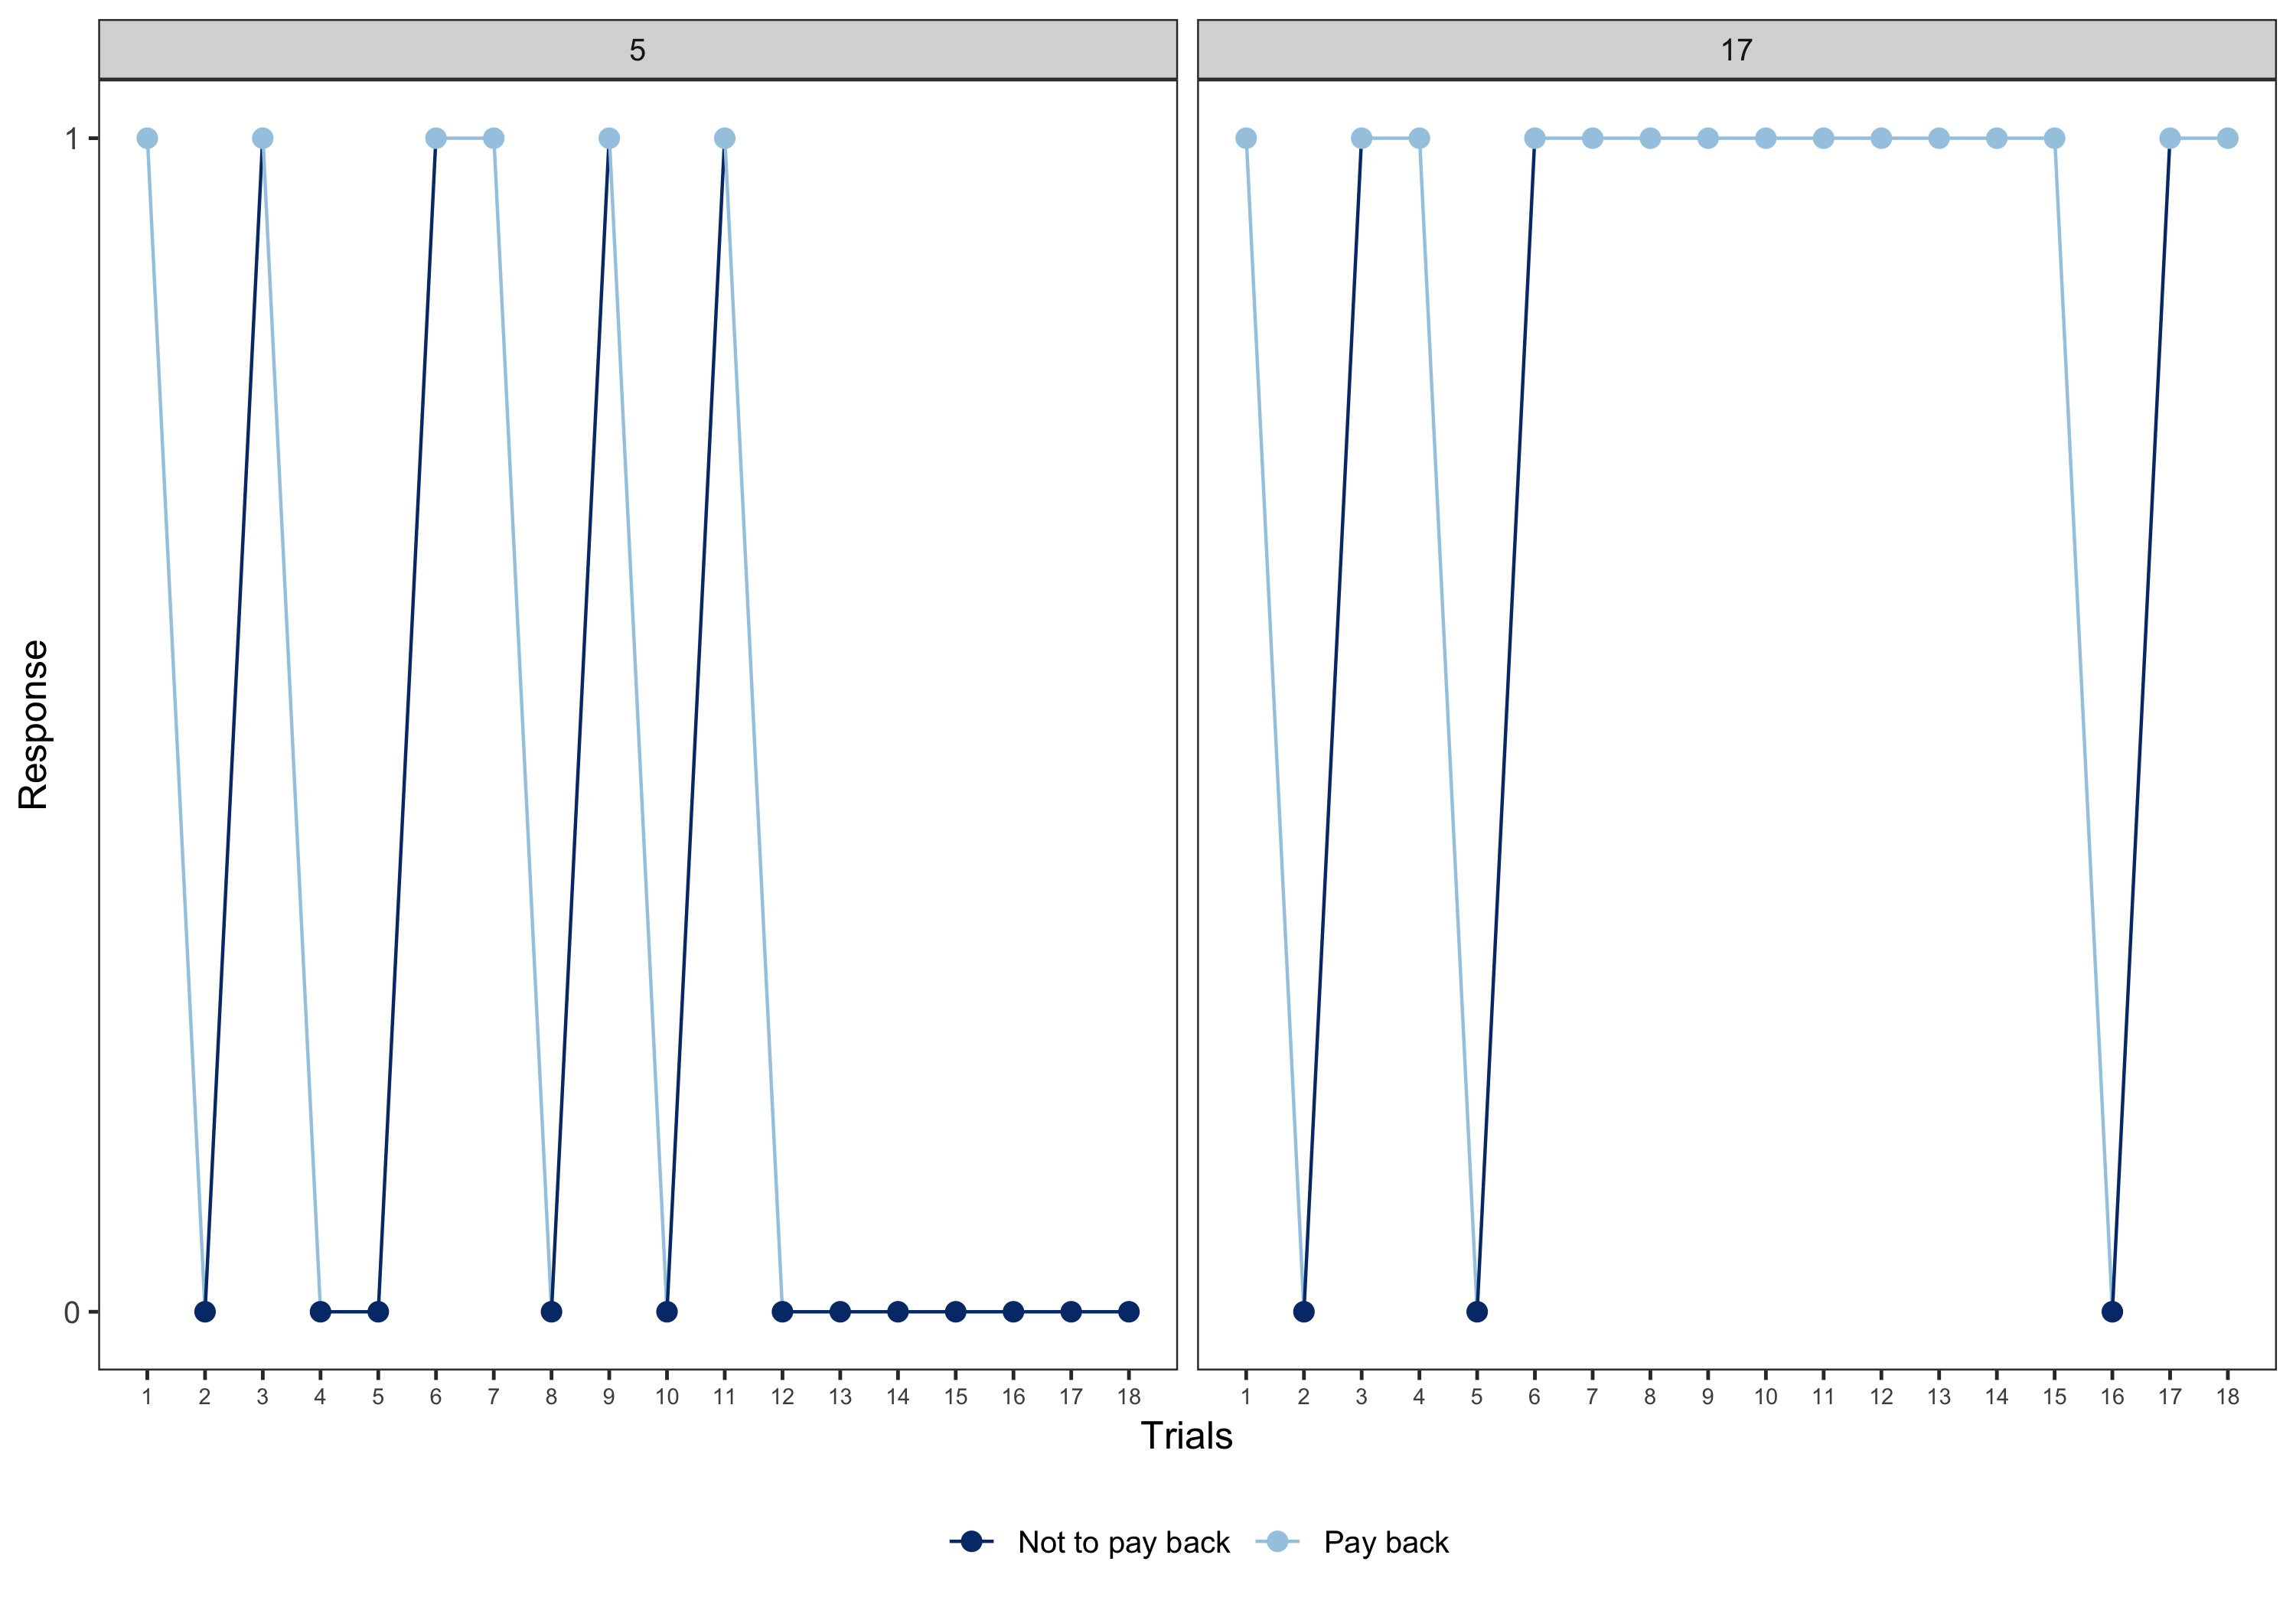
\includegraphics[width=0.8\linewidth]{/Users/saidjimenez/Documents/R/github_Said/social_closeness/Manuscript/figures/g10} 

}

\caption{Subjects from two latent thetas}\label{fig:g10}
\end{figure}

\begin{figure}

{\centering 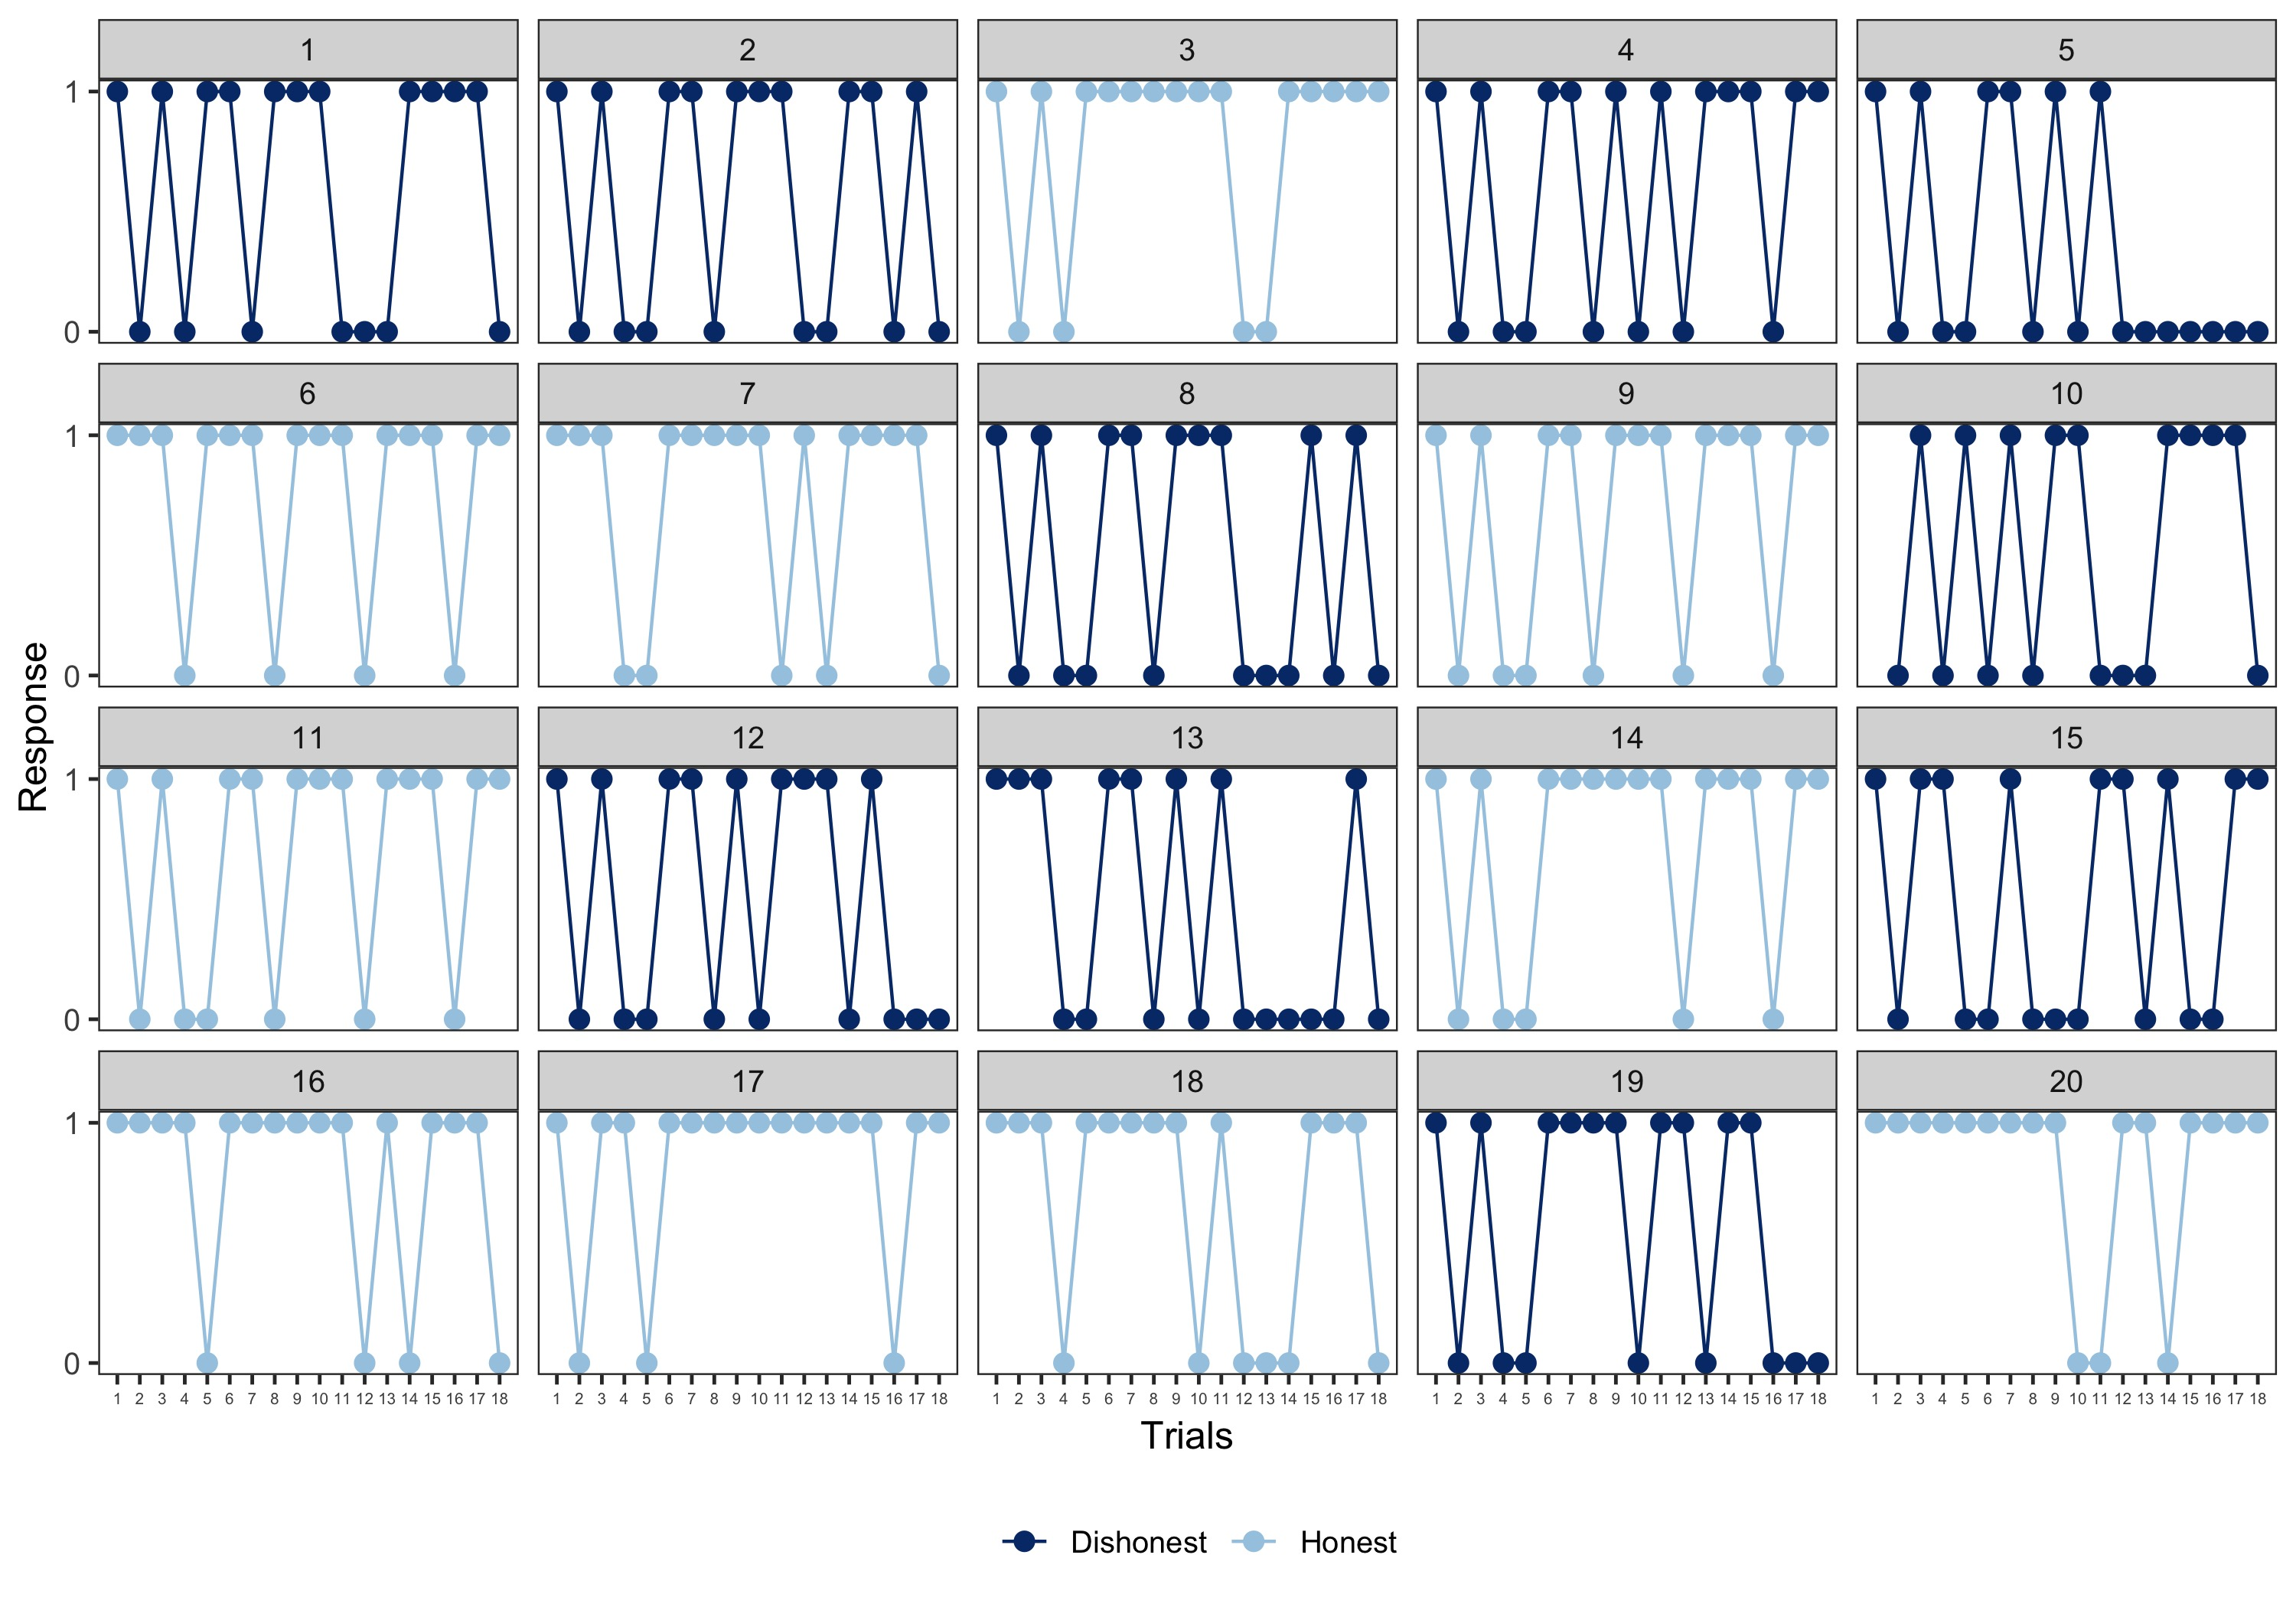
\includegraphics[width=0.8\linewidth]{/Users/saidjimenez/Documents/R/github_Said/social_closeness/Manuscript/figures/g11} 

}

\caption{Strategies by group}\label{fig:g11}
\end{figure}

\begin{figure}

{\centering 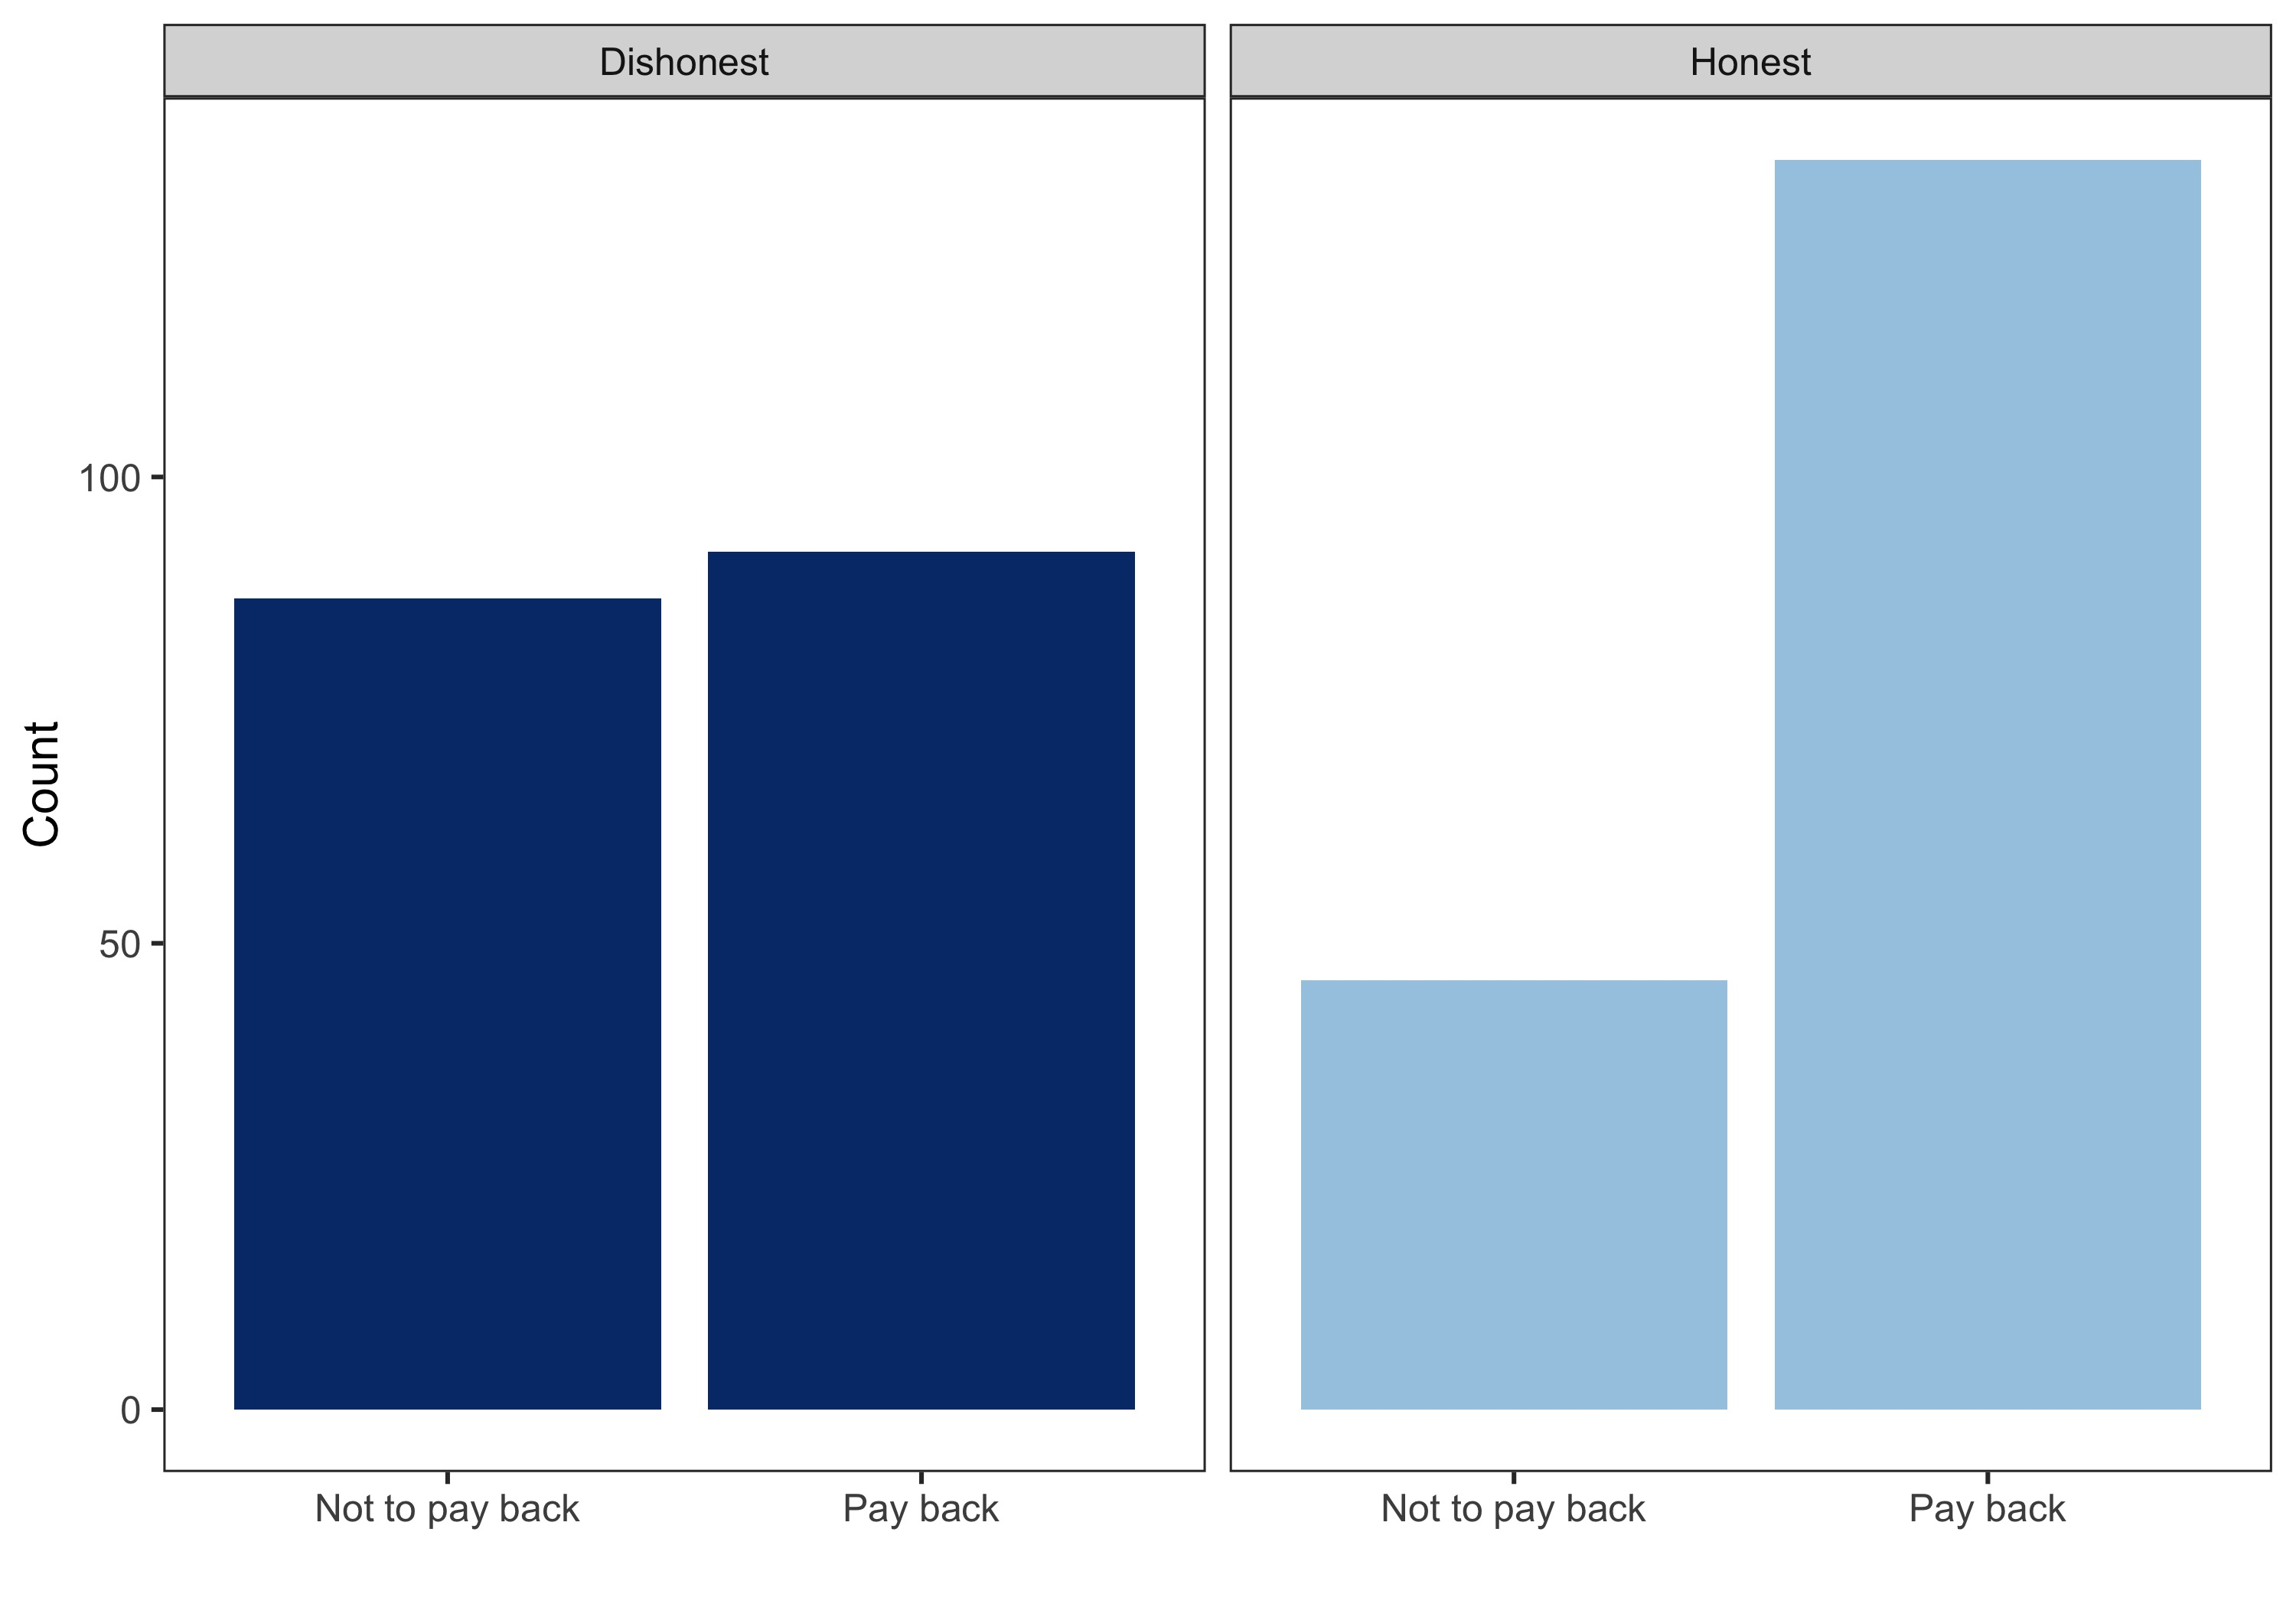
\includegraphics[width=0.8\linewidth]{/Users/saidjimenez/Documents/R/github_Said/social_closeness/Manuscript/figures/g12} 

}

\caption{Rates by group}\label{fig:g12}
\end{figure}

\begin{figure}

{\centering 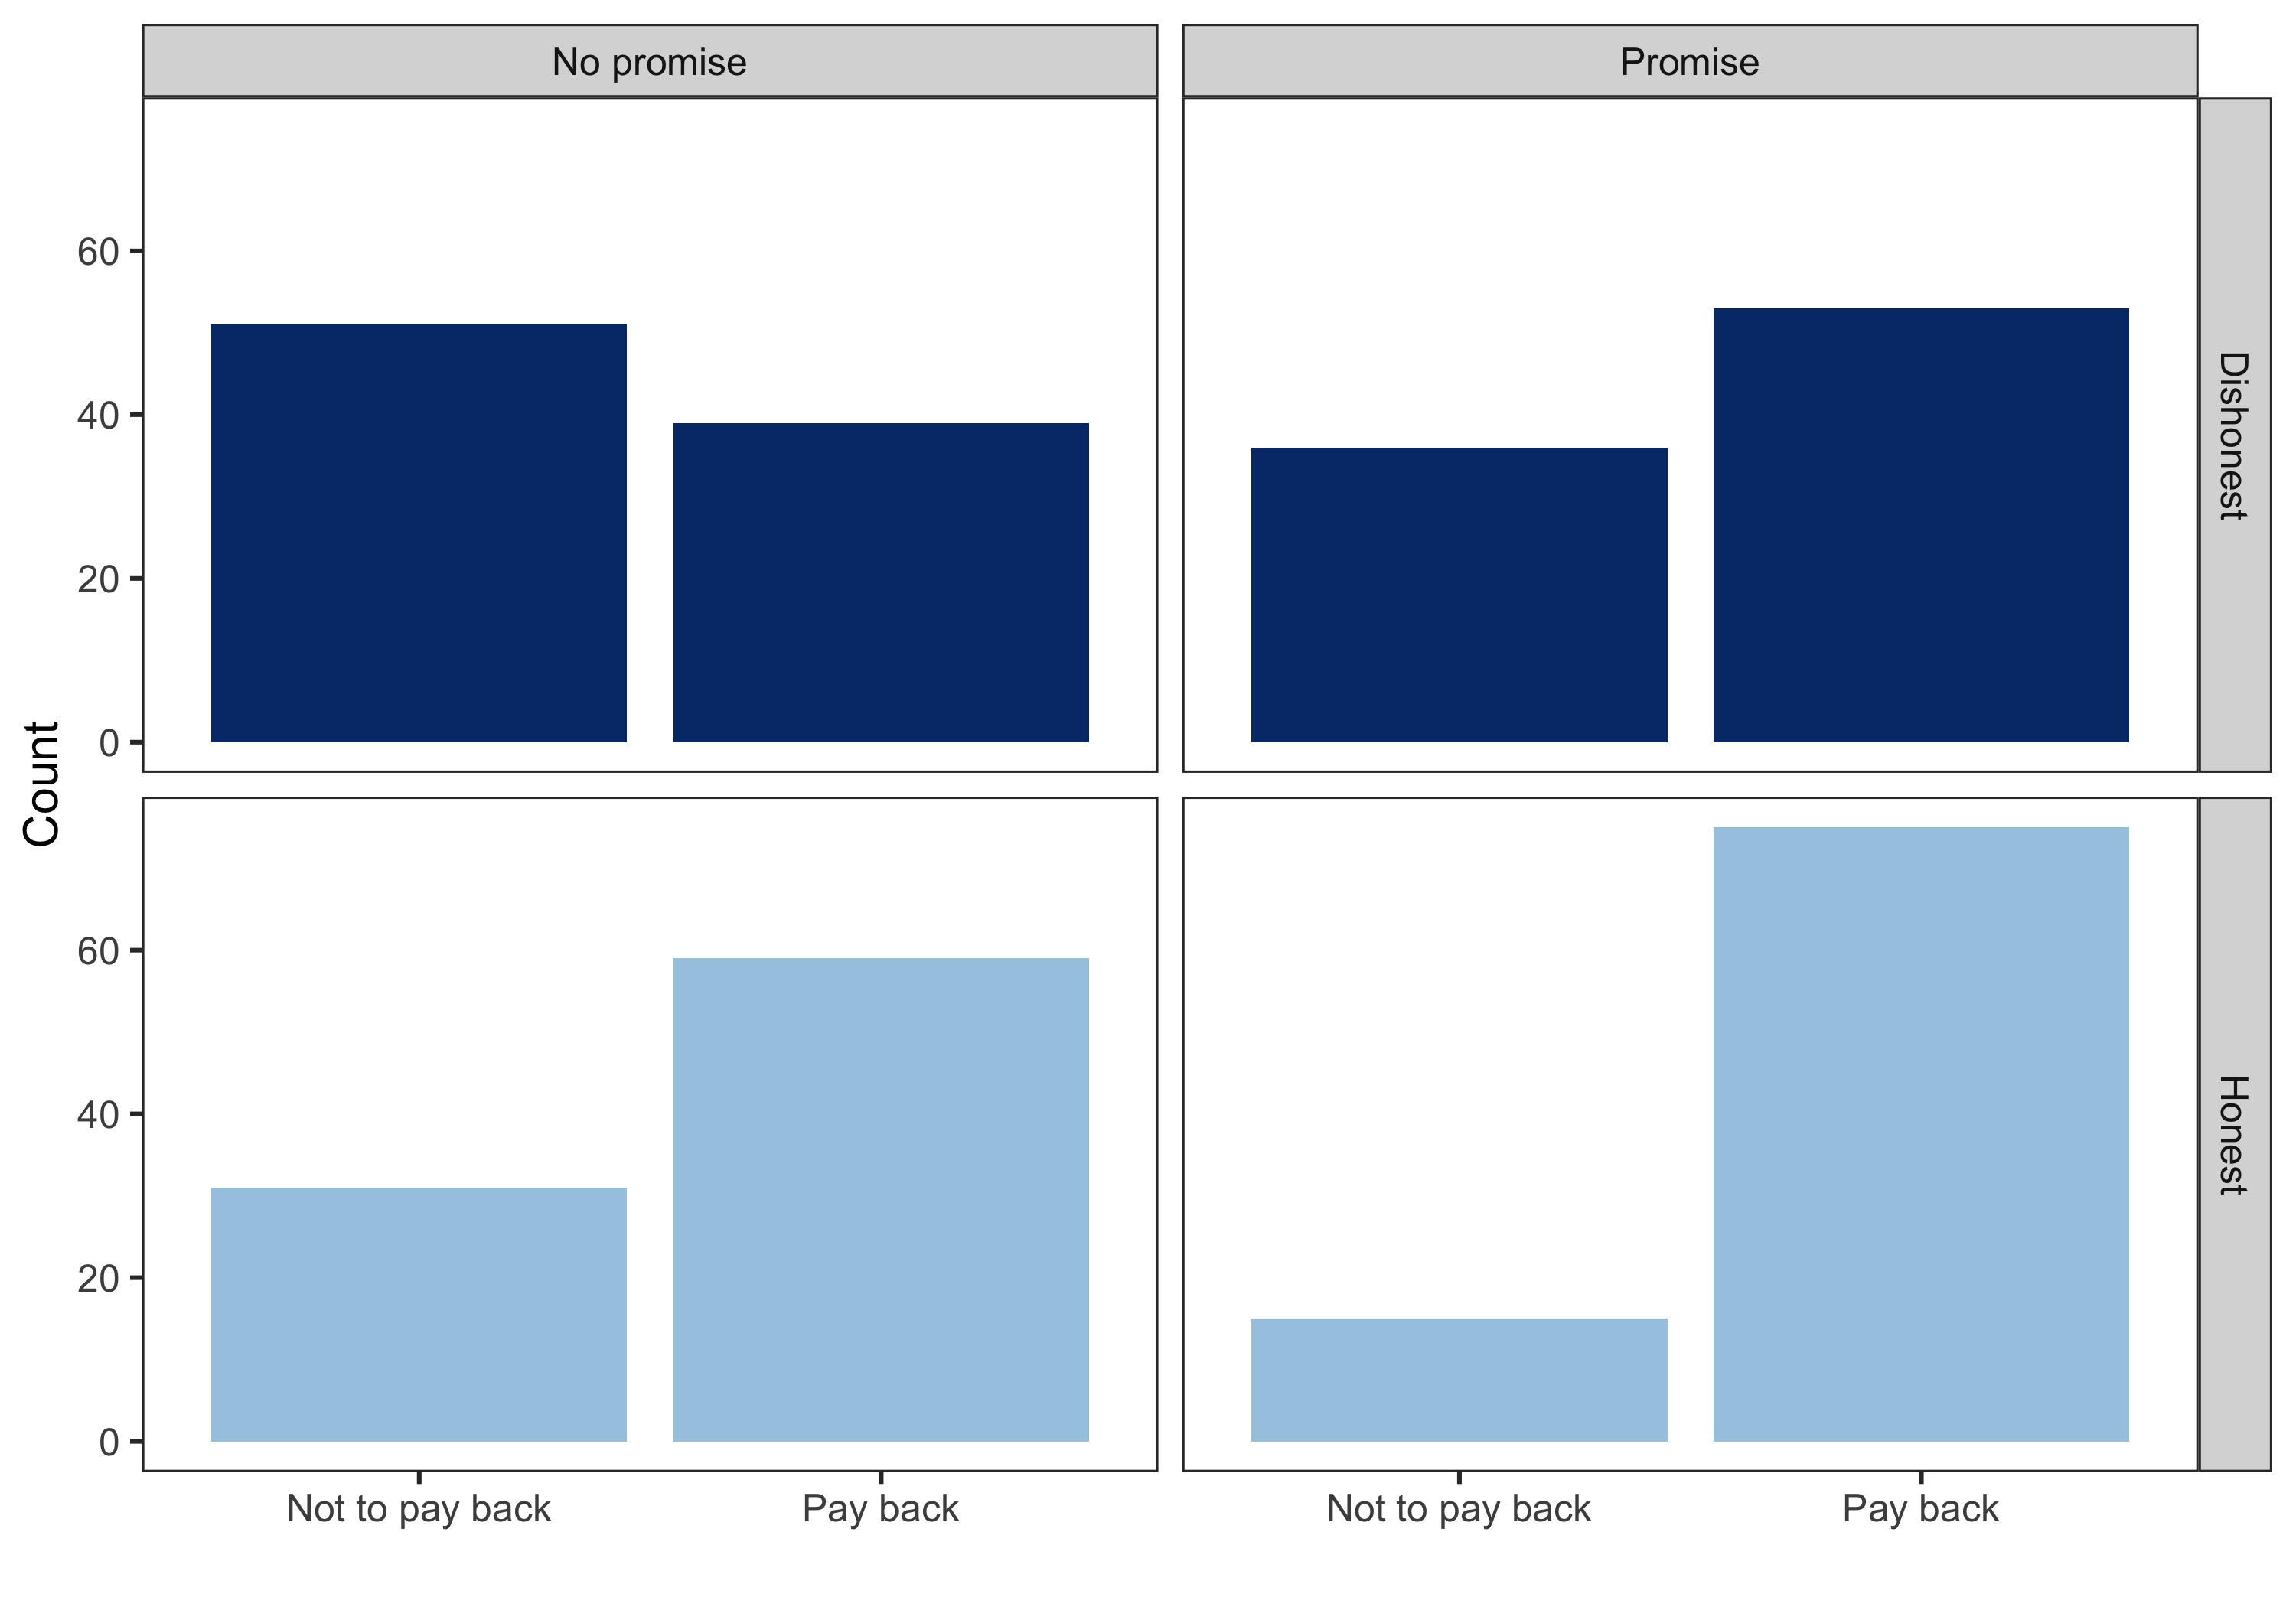
\includegraphics[width=0.8\linewidth]{/Users/saidjimenez/Documents/R/github_Said/social_closeness/Manuscript/figures/g12_b} 

}

\caption{Rates by group and promise condition}\label{fig:g12_b}
\end{figure}

\begin{figure}

{\centering 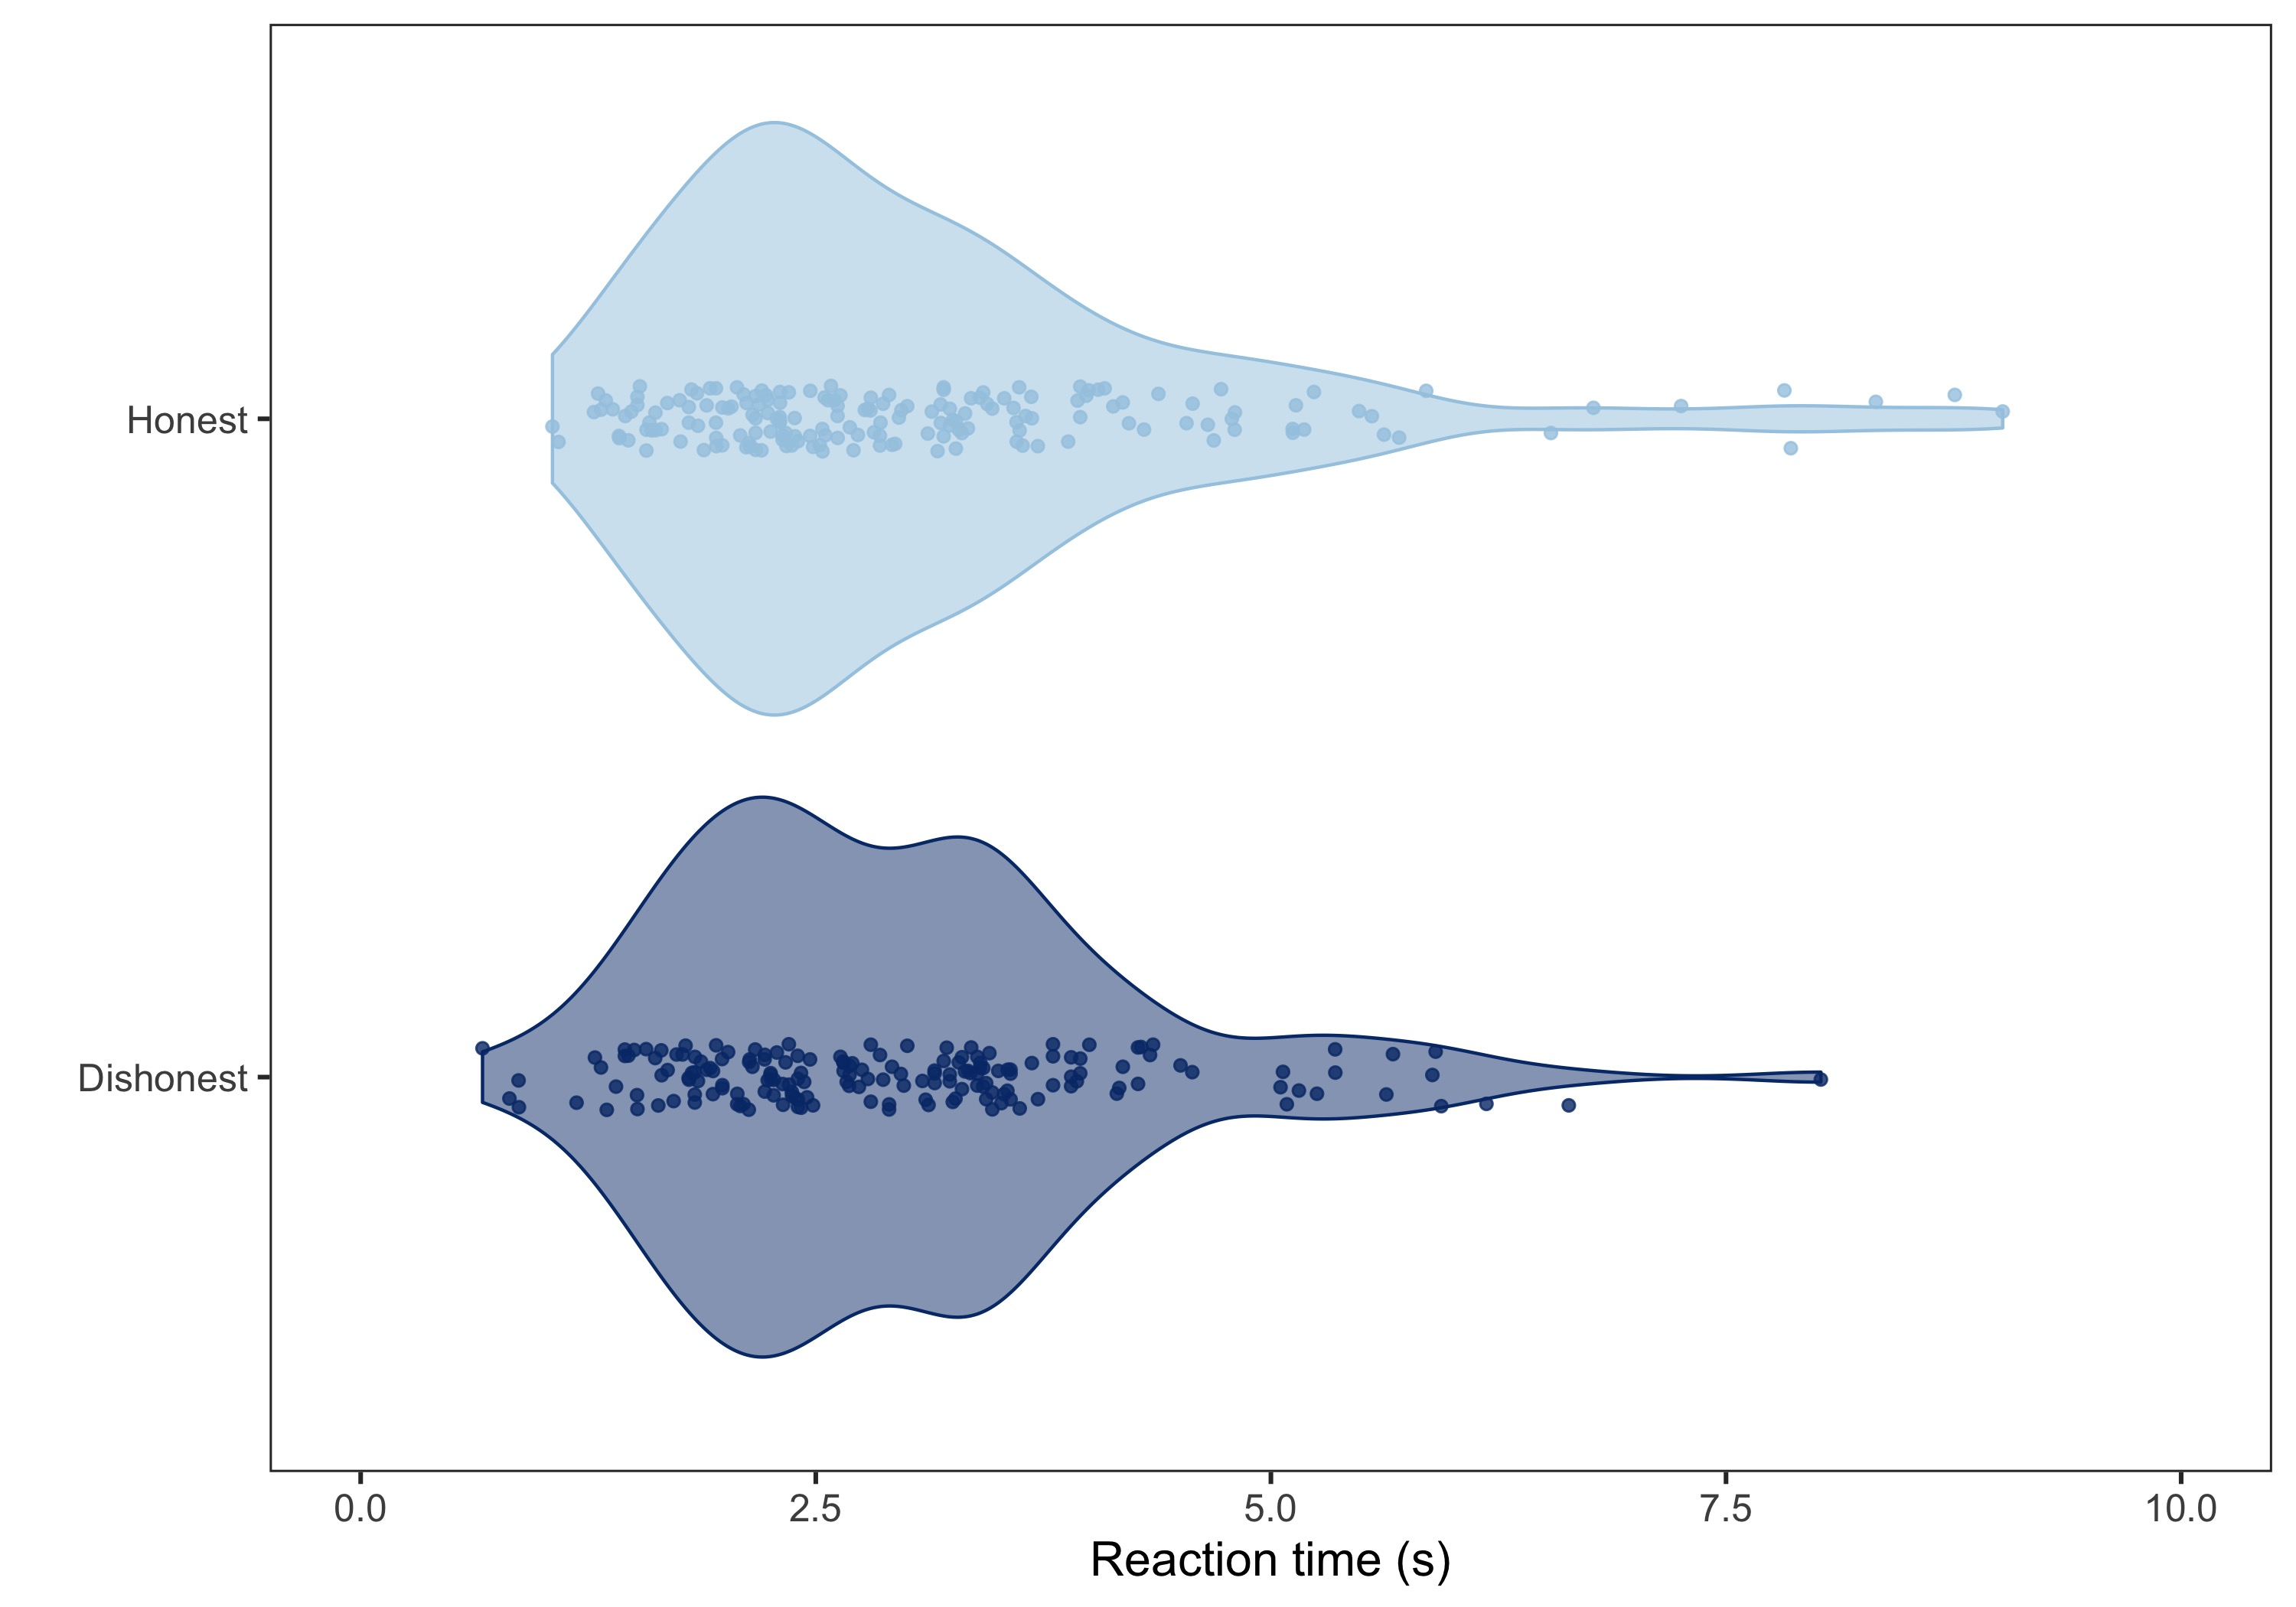
\includegraphics[width=0.8\linewidth]{/Users/saidjimenez/Documents/R/github_Said/social_closeness/Manuscript/figures/g13} 

}

\caption{Reaction times by group}\label{fig:g13}
\end{figure}

\begin{figure}

{\centering 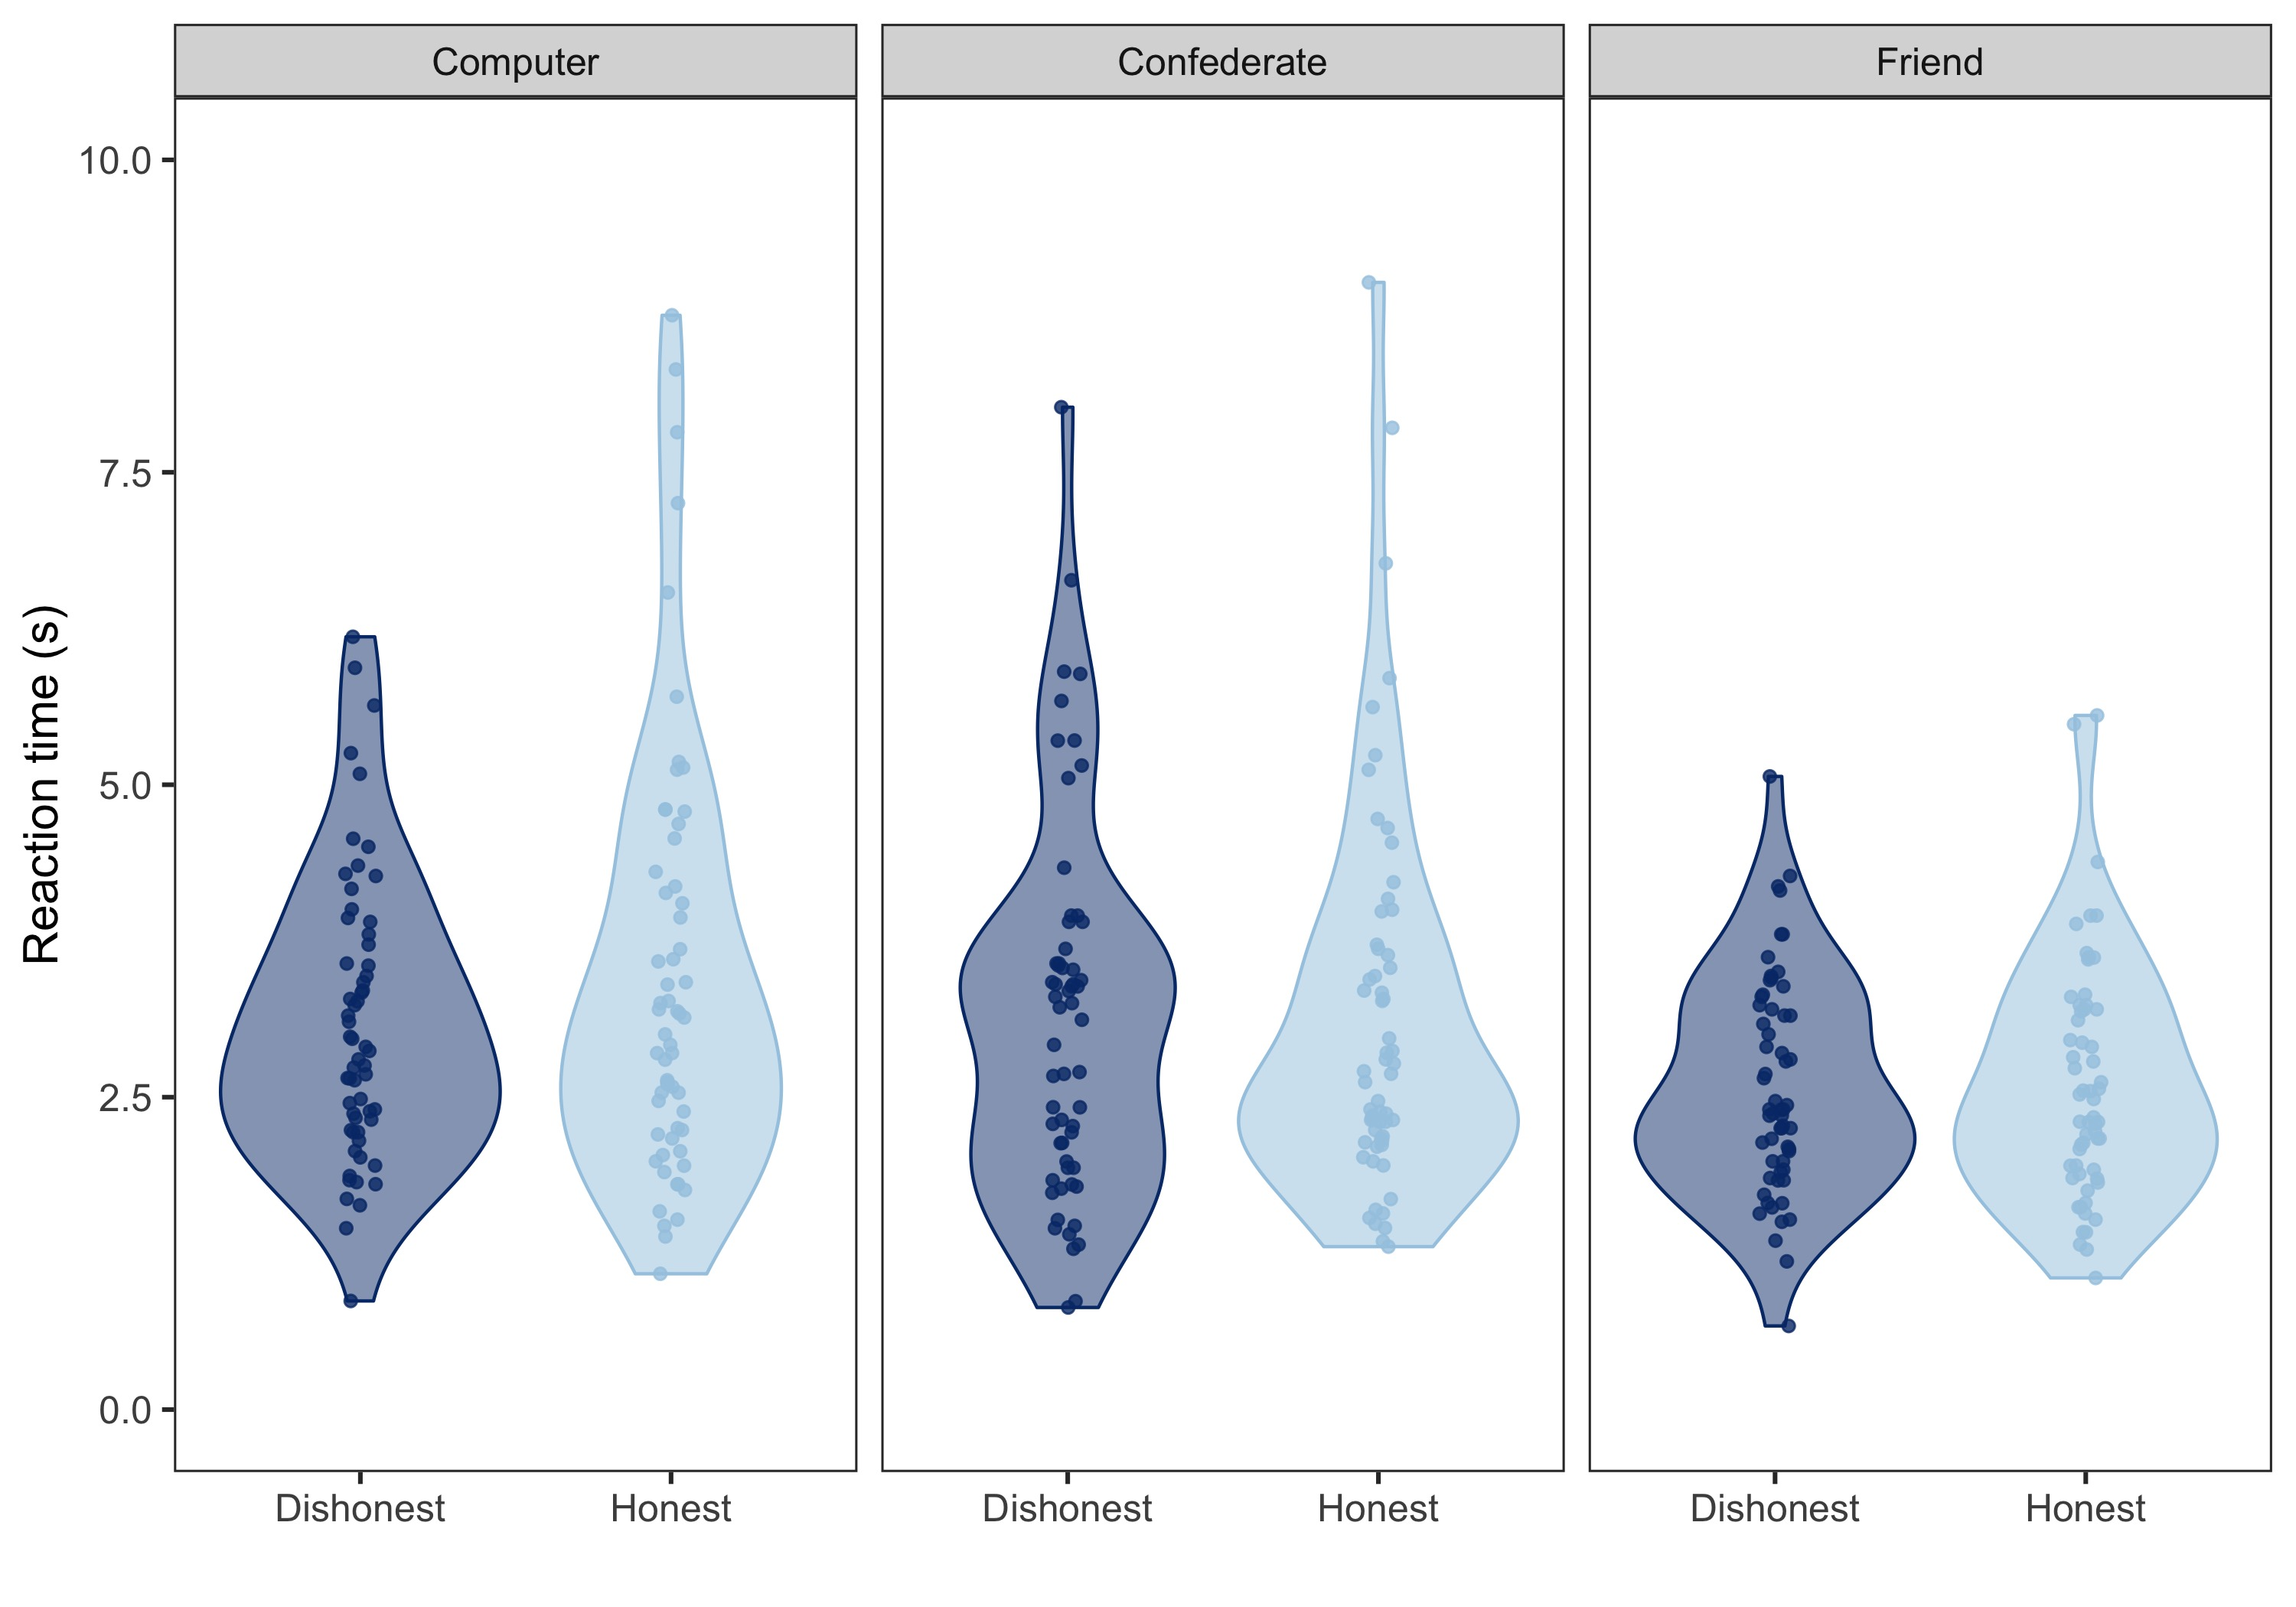
\includegraphics[width=0.8\linewidth]{/Users/saidjimenez/Documents/R/github_Said/social_closeness/Manuscript/figures/g14} 

}

\caption{Reaction times by partner}\label{fig:g14}
\end{figure}

\begin{figure}

{\centering 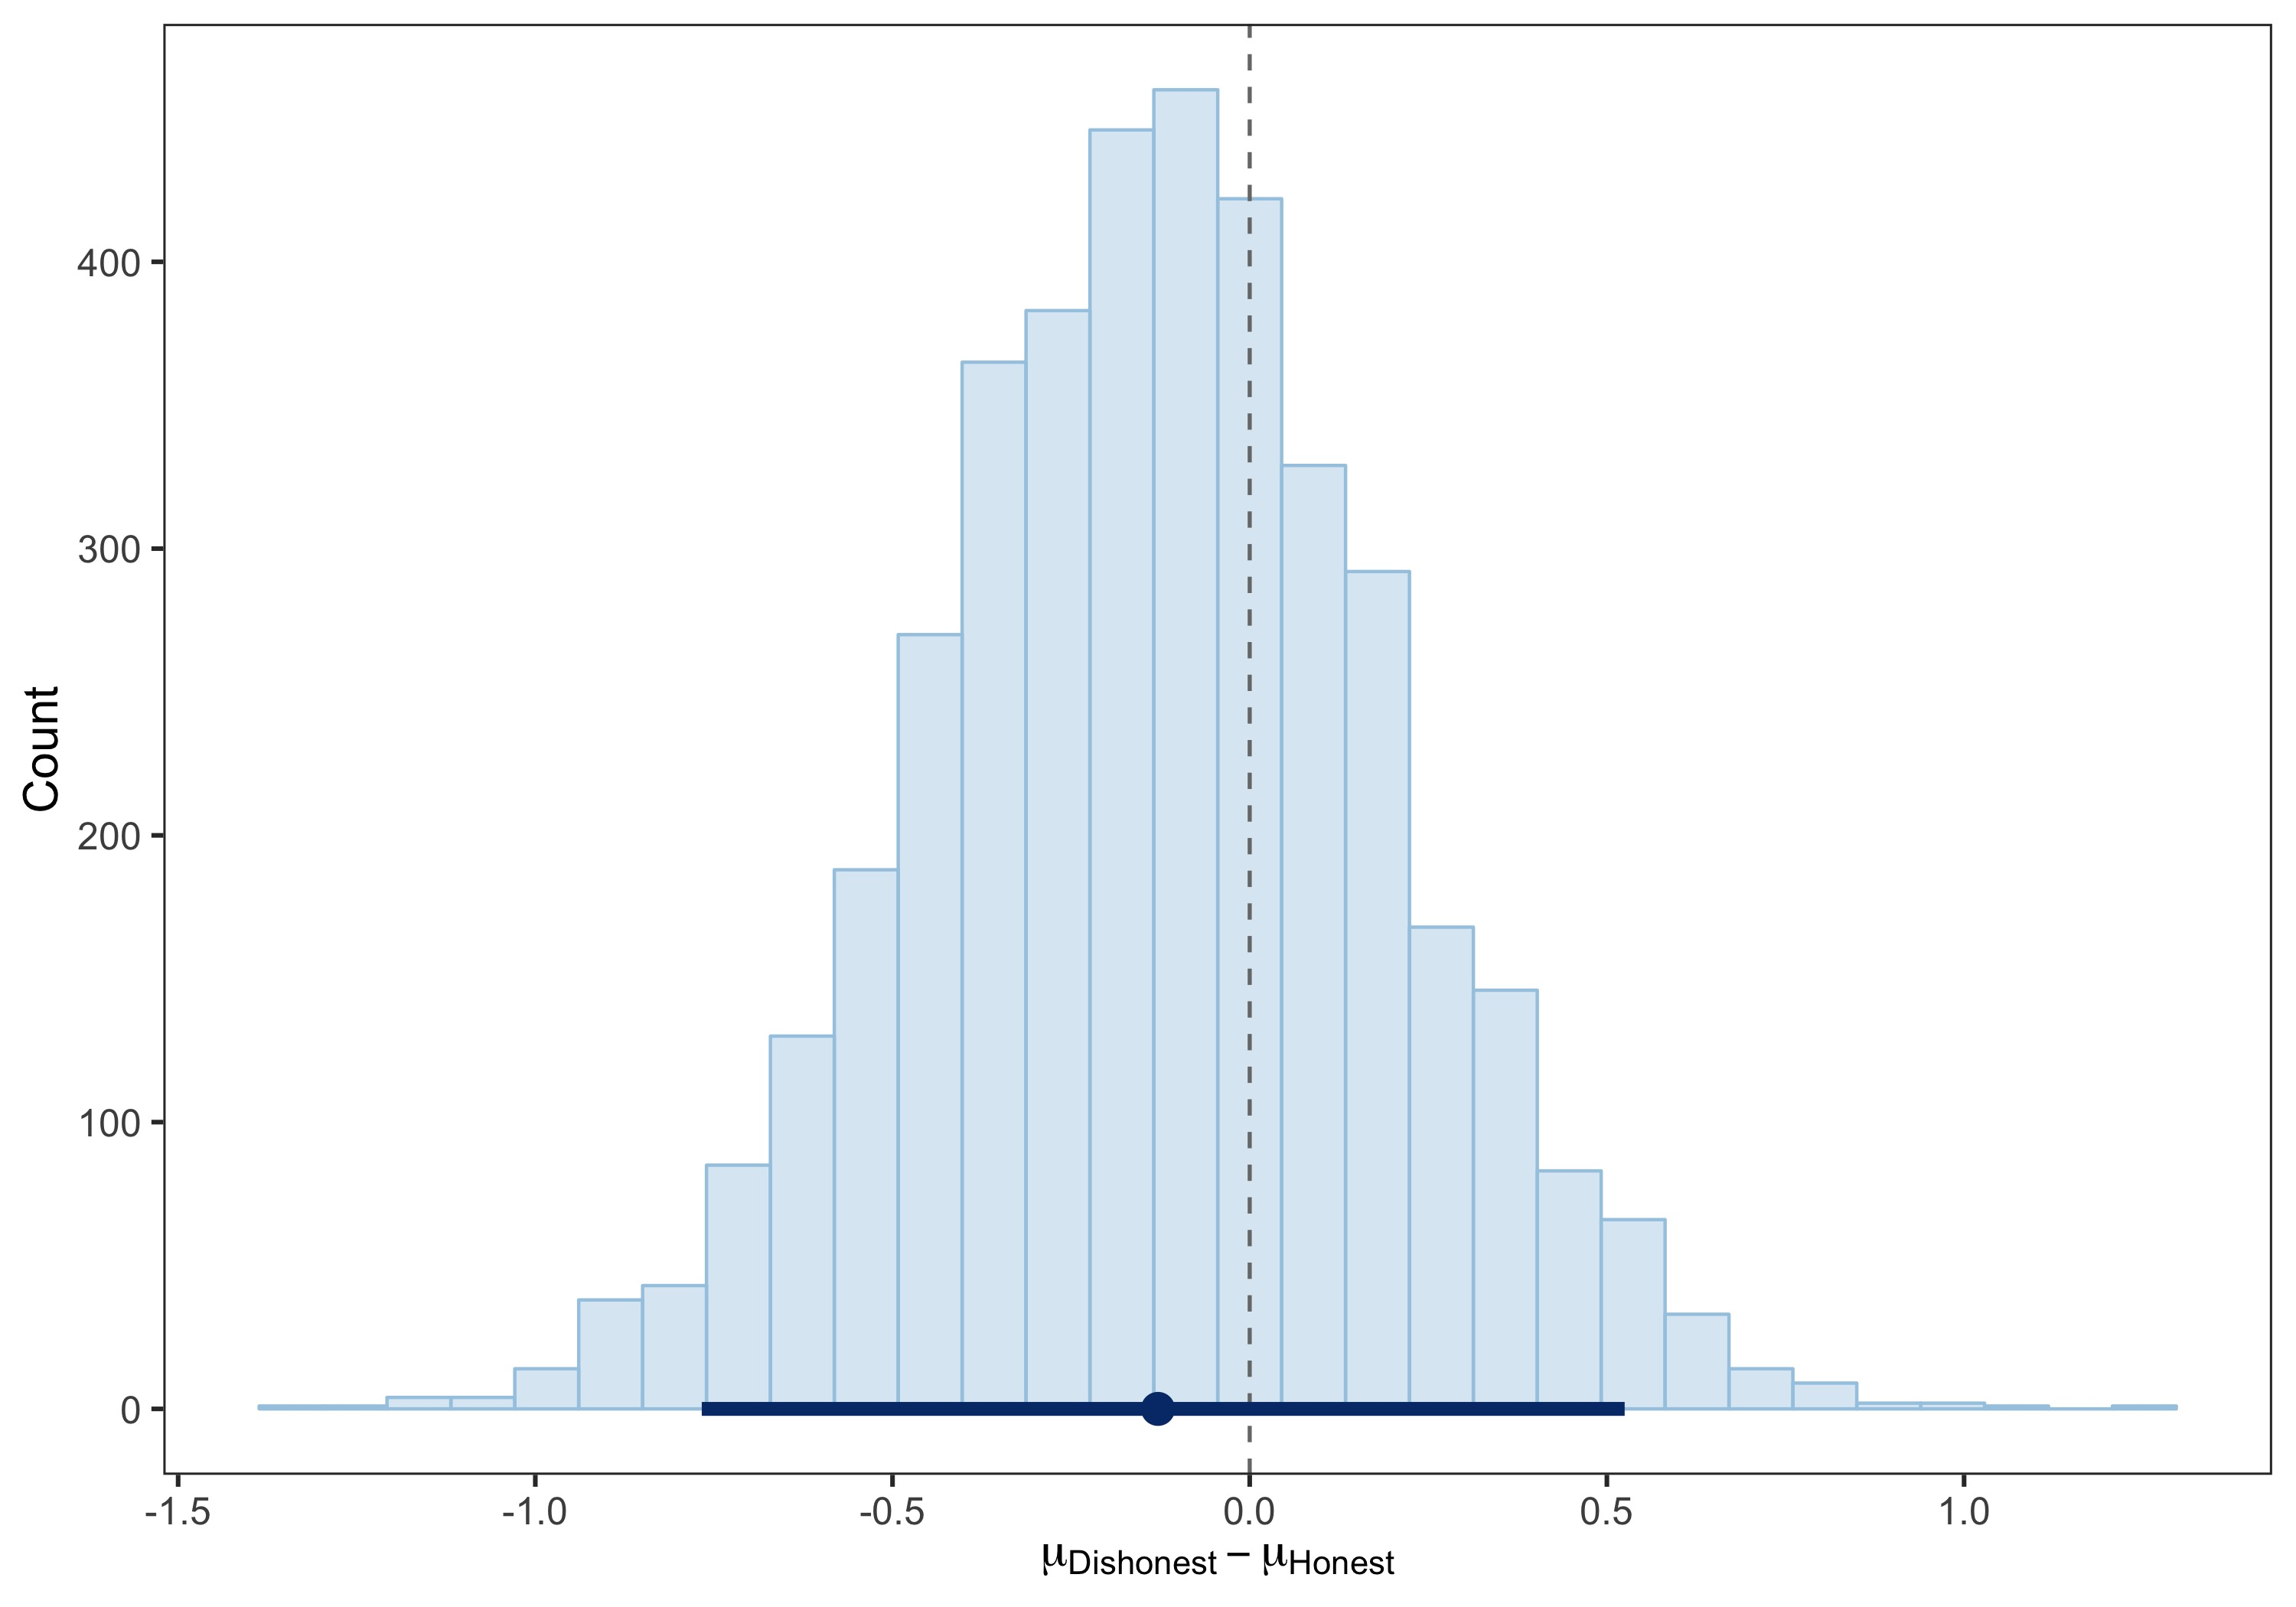
\includegraphics[width=0.8\linewidth]{/Users/saidjimenez/Documents/R/github_Said/social_closeness/Manuscript/figures/g15} 

}

\caption{Difference between groups in reaction time}\label{fig:g15}
\end{figure}
\newpage
\singlespacing 
\bibliography{\textasciitilde{}/Dropbox/master.bib}
\end{document}



